% Prelim, Chapter 4
% by Rachel Slaybaugh

\chapter{Preconditioning}
\label{sec:Chp4}
The new ``grand challenge'' problems facing the nuclear transport community are large and complex. Cutting edge methods are required to solve them. While the second and third chapters discussed new methods that enable the solution of such problems, low-cost preconditioners that can reduce the number of iterations needed for convergence will be invaluable. In Benzi et.\ al.'s 2002 survey paper on preconditioning techniques for large linear systems they state ``it is widely recognized that preconditioning is the most critical ingredient in the development of efficient solvers for challenging problems in scientific computation \cite{Benzi2002}.'' 

This is true for Krylov methods in particular because the memory required and cost per iteration increase dramatically with the number of iterations \cite{Benzi2002}. And, as discussed in Chapter \ref{sec:Chp3}, Krylov methods can converge very slowly for poorly conditioned systems. When this happens the eigenvector is not converged in a reasonable number of iterations and RQI cannot converge the eigenvalue. Preconditioning is therefore required to make RQI useful. 

This chapter is about the new preconditioner added to Denovo. First some background information that includes an introduction to preconditioning, an overview of preconditioners used in the nuclear community, and a discussion of multigrid methods is given. Next, past and related work is discussed. Finally the new preconditioner is explained, and results demonstrating its impact are given. 

%-------------------------------------------------------------------------------------------
%-------------------------------------------------------------------------------------------
\section{Background}
The general idea of preconditioning is to transform the system of interest into another equivalent system that has more favorable properties, for example one with a smaller condition number. A preconditioner is a matrix that induces such a transformation by improving the spectral properties of the problem being solved. Let $\ve{G}$ be a non-singular preconditioner, then $\ve{A}x=b$ can be transformed in the following ways \cite{Benzi2002}: 
%
\begin{alignat}{3}
  \ve{G}^{-1}\ve{A}x &= \ve{G}^{-1}b  &  &\text{left preconditioning,} \\
  \ve{AG}^{-1}y &= b, \qquad  &x = \ve{G}^{-1}y \qquad &\text{right preconditioning, and } \\
  \ve{G}_{1}^{-1}\ve{AG}_{2}^{-1}y &= \ve{G}_{1}^{-1}b, \qquad \ve{G} = \ve{G}_{1}\ve{G}_{2}, \qquad  &x = \ve{G}_{2}^{-1}y  \qquad &\text{split preconditioning.} 
\end{alignat}

If $\ve{A}$ and/or $\ve{G}$ are non-normal then each of the preconditioning constructs will likely give different behavior, though they will converge to the same answer because the matrices are similar and therefore have the same eigenvalues  \cite{Benzi2002}. Right preconditioning leaves the right hand side of the equation unaffected and does not change the norm of the residual, which is used for convergence testing in most iterative methods. Right preconditioning is usually preferred over left preconditioning for iterative solvers for this reason \cite{Knoll2004}. A right preconditioner was implemented in this work, and the remaining discussion will be presented in right preconditioner format. 

There are two extremes between which all other preconditioners lie: $\ve{G} = \ve{A}$, in which case the solution can be found directly, and $\ve{G} = \ve{I}$, which will have no effect. The matrix $\ve{A}\ve{G}^{-1}$ is not formed in practice. The preconditioner can be applied by using some method to solve $\ve{G}y=c \to y \approx \ve{G}^{-1}c$, or by otherwise implementing the action of $\ve{G}^{-1}$ without ever explicitly forming and inverting $\ve{G}$ \cite{Benzi2002}, \cite{Trefethen1997}. 

Functionally, a good preconditioner should make the system easier to solve and result in faster convergence. It should also be cheap to construct and apply. These tend to be competing goals in that the easier a preconditioner is to construct and apply the less it typically does to improve convergence. A preconditioner is considered good if $\ve{A}\ve{G}^{-1}$ is not too far from normal and its eigenvalues are clustered \cite{Trefethen1997}. 

There are many different types of preconditioners, but they can be put into two general categories: matrix-based and physics-based. Matrix-based preconditioners rely entirely on the structure of the matrix $\ve{A}$ regardless of the physics going on in the problem. That is, these methods do not change when the underlying problem changes. This can be a very useful property because matrix-based methods are then broadly applicable and do not require any understanding of the physical problem. Extrapolation methods and incomplete factorizations are examples of a matrix-based preconditioners \cite{Trefethen1997}.

Physics-based preconditioning uses knowledge about the physics of the problem in question to guide the creation of the preconditioner. This means that some methods only work with certain kinds of problems, and that the preconditioners may have to be tailored or adapted for different applications. However, such methods take advantage of knowing something about the problem and can be more effective than matrix-based methods for the range of problems for which they are intended. Rebalance and synthetic acceleration are examples of physics-based preconditioners \cite{Trefethen1997}.

%-----------------------------------------------------------------------------------------------
\subsection{Preconditioners in the Nuclear Community}
A variety of acceleration methods have been used by the nuclear computational community over the years. This subsection gives a high-level overview of some common methods. In 2002 Adams and Larsen put together a comprehensive overview of the development of iterative methods for solving the \Sn transport equation \cite{Adams2002}. For more detail and history about each method, refer to this publication. 

\subsubsection{Extrapolation Methods}
Extrapolation methods were historically used to accelerate $k$-eigenvalue calculations. These tend to be based on simple iterative solvers or polynomial approximations. One step of a simple iterative method such as Jacobi, Gauss Seidel, or successive over relaxation (SOR) can be used at the outset of a problem to serve as a preconditioner \cite{Trefethen1997}. When applied to neutron transport, an overrelaxation method looks like $\ve{F}_{i+1} = \omega(\tilde{\ve{F}}_i - \ve{F}_i) + \ve{F}_i$ with $1 \le \omega < 2$, where the unaccelerated new iterate for the fission source is designated $\tilde{\ve{F}}_i$ \cite{Lewis1993}.

Polynomial preconditioners create a matrix polynomial $\ve{G}^{-1} = p(\ve{A})$, where $p(\ve{A})$ serves as a polynomial approximation to $\ve{A}^{-1}$. Common polynomial choices are truncated Neumann series and Chebyshev polynomials. An advanced variation of this method is to determine the polynomial coefficients adaptively \cite{Trefethen1997}. When Chebyshev polynomials are applied to the transport equation, $\ve{F}_{i+1} = \ve{F}_i + \alpha_{i+1}(\tilde{\ve{F}}_i - \ve{F}_i) + \beta_i(\ve{F}_i - \ve{F}_{i-1})$, where $\alpha$ and $\beta$ are iteration dependent \cite{Lewis1993}. Neither of these extrapolation methods are widely used today as they have not been very successful in multi-dimensional problems. There are analogous versions of these methods for fixed source problems \cite{Alcouffe1977}.  

\subsubsection{Rebalance}
Rebalance methods are designed to accelerate iteration on the scattering or fission source by imposing a balance condition on the unconverged solution over either coarse or fine regions. If the region is coarse, this is a coarse-grid approximation preconditioner since fine-grid physics are excluded. If the region is fine, this is a local approximation preconditioner where short range effects are permitted and long range interactions are excluded \cite{Trefethen1997}, \cite{Adams2002}.

In either case, the unaccelerated solution is multiplied by a constant in each region that satisfies the balance equation. The rebalance process adjusts the average amplitude of the flux over a region and the iteration adjusts the space-angle distribution. The notion is that these processes work in concert to eliminate all error modes simultaneously \cite{Adams2002}. 

Coarse mesh rebalance (CMR) has been more successful than the fine version and is therefore used more often. In practice, choosing regions properly must be done with care \cite{Lewis1993}. Traditional forms of CMR can be unstable for problems where the spatial mesh is large compared to the neutron mean-free-path and where the scattering ratio is close to unity \cite{Alcouffe1977}. 

\subsubsection{Incomplete Factorizations}
Incomplete factorization methods were first introduced in the 1950s by Buleev, and independently by Varga. In the late 1970s these methods started gaining popularity, and since then have been under active development. The idea is to partially factor the matrix $\ve{A}$ such that the resulting matrices are sparse enough to take advantage of sparse solver methods, but close enough to $\ve{A}$ to be valuable as preconditioners \cite{Benzi2002}.

Incomplete Cholesky (IC) or incomplete LU (ILU) factorization have both been extensively used within the nuclear community. The Cholesky version is used when $\ve{A}$ is symmetric and LU when non-symmetric. Factorizations typically destroy sparsity, resulting in matrices that are denser than the originals and making their use more costly. Different variations of incomplete factorization methods address this by permitting the new matrices to have values only in positions where $\ve{A}$ has values, allowing a prescribed amount of fill in or only saving entries greater than some tolerance \cite{Trefethen1997}, \cite{Patton2002}, \cite{Oliveira1998}.

\subsubsection{Synthetic Acceleration}
In synthetic acceleration a low-order approximation to the transport operator is used to accelerate the full transport problem \cite{Lewis1993}. If a system is discretized with a high-order method it can be preconditioned with a lower-order approximation. The low-order method is often much sparser than the original, but still captures the general behavior of the problem \cite{Trefethen1997}. This is generally done with either the diffusion equation, giving diffusion synthetic acceleration (DSA), or a transport equation  that is simpler than the one actually being solved, giving transport synthetic acceleration (TSA). These can be used for fission or fixed source problems \cite{Adams2002}. 

%Synthetic methods have at least two iteration stages. The simplest way to illustrate this is to use source iteration for the within-group solver. The first step is a transport sweep, giving:
%%
%\begin{equation}
%  \ve{L}\psi^{(l+\frac{1}{2})} = \ve{S}\psi^{(l)} + q \:, \qquad l \ge 0 \:.
%  \label{eq:synthetic}
%\end{equation}
%%
%Here $l$ is the iteration index, $\ve{L}$ is the transport operator, $\ve{S}$ is the scattering matrix, and $q$ is the external source. Equation \eqref{eq:synthetic} is subtracted from the exact equation to get an expression for an exact additive correction:
%%
%\begin{equation}
%  \bigl( \ve{L} - \ve{S} \bigr)\bigl( \psi - \psi^{(l+\frac{1}{2})} \bigr) = \ve{S}\bigl(\psi^{(l+\frac{1}{2})} - \psi^{(l)} \bigr) \:.
%  \label{eq:correction}
%\end{equation}
%%
%This cannot be solved exactly, but the idea of synthetic methods is to find an $\ve{G}^{-1} \approx (\ve{L} - \ve{S})^{-1}$ that will be easier to evaluate than $(\ve{L} - \ve{S})^{-1}$. Equation \eqref{eq:synthetic} is solved by a high-order scheme and Equation \eqref{eq:correction} is solved with a low-order approximation. If the synthetic system converges, it must satisfy the original transport equation \cite{Adams2002}. 

Original DSA formulations exhibited instability in some instances. In 1977 Alcouffe demonstrated with diamond difference that stability can be obtained by using a consistent spatial differencing scheme \cite{Alcouffe1977}. The transport and diffusion equations cannot be discretized independently or the diffusion equation may not satisfy the original transport equation. The discretization of the diffusion equation must therefore be derived from the discretization of the transport equation such that they are consistent. Alcouffe's idea has since been extended to accelerate currents, to more dimensions, and to different spatial discretizations \cite{Larsen1982}. 

DSA can be implemented a few different ways, each of which performs a transport sweep and then solves a corrected diffusion equation. Different terms in the diffusion equation can be corrected for different problem types \cite{Alcouffe1977}. DSA has been found to degrade in the presence of material discontinuities in addition to when it is not consistently derived. However, Warsa et.\ al.\ found that when DSA is used as a preconditioner for Krylov iterative methods, it is effective even when only partially consistent \cite{Warsa2004}.

To address the concerns about spatial discretization associated with DSA, a low-order transport solve could be used to find the correction term instead. Larsen and Miller developed a method that neglects scattering in the low-order transport equation, but this can cause instability in multi-dimensional problems. Ramone et.\ al.\ proposed including some scattering by using a tunable parameter. A high-order transport equation is solved first, then a transport equation with a coarse quadrature and reduced scattering is solved to find the correction that is applied to the new iterate of the scalar flux \cite{Ramone1997}. This algorithm can be viewed as Richardson iteration with a coarse operator preconditioner. Synthetic acceleration methods are widely used and actively researched in the transport community today.

%-----------------------------------------------------------------------------------------------------
\subsection{Multigrid Methods}
The new preconditioner added to Denovo does multigrid in the energy dimension. To understand why multigrid in energy makes sense, why multigrid methods work must be understood. The material presented here is largely from \emph{A Multigrid Tutorial} by Briggs, Henson, and McCormick \cite{Briggs2000}, supplemented by Dr. Strang's lectures on multigrid and preconditioners available as MIT Open Courseware \cite{Strang}.

In what follows, the system of equations will be denoted as $\ve{A}u=b$ where $u$ will represent the exact solution and $v$ will indicate the approximate solution. The algebraic error is given by $e = u - v$. Since $e$ cannot be calculated exactly (otherwise the answer would be known), the residual, $r = b - \ve{A}v$ is often used. A certain grid will be denoted as $\Omega^{h}$ where $h$ is the grid spacing, and vectors on that grid are $u^{h}$. 

The error in any guess can be written as a combination of Fourier modes. A Fourier mode is described by a wavenumber, $k$, which denotes the frequency of oscillation. The $j$th Fourier mode is 
% 
\begin{equation}
    e_{j} = \sin\bigl(\frac{jk\pi}{n}\bigr) \:, \qquad 0 \le j \le n \:, \qquad 1 \le k \le n-1 \:.
\end{equation} 
%
There are $k$ half sine waves that comprise $e$ on the domain of the problem. The term $e_{k}$ indicates an $e$ with wavenumber $k$. The $k$th wave has $\frac{k}{2}$ full sine waves with a wavelength of $\frac{2}{k}$. Modes with wavenumbers in the range $1 \le k \le \frac{n}{2}$ are called low-frequency or smooth modes and those in $\frac{n}{2} \le k \le n-1$ are called high-frequency or oscillatory modes. Figure \ref{fig:FourierModes} shows what a few different modes look like. 
%
\begin{figure}[!ht]
    \begin{center}
      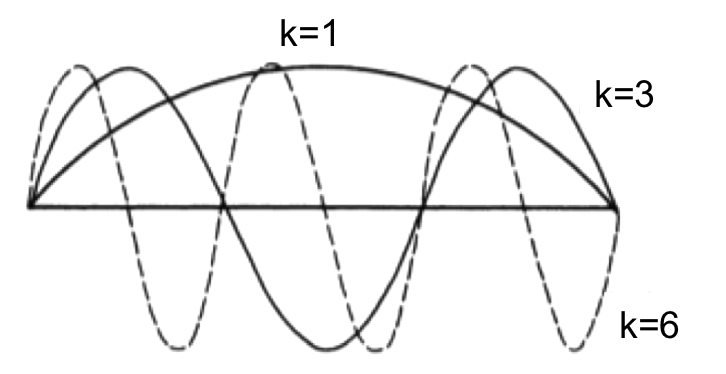
\includegraphics [width=0.45\textwidth, height=0.2\textheight] {FourierModes}
   \end{center}
   \caption{Three Fourier Modes \cite{Briggs2000}}
   \label{fig:FourierModes}
\end{figure}

Iterative methods, also referred to as smoothers or relaxers, remove high frequency error components very quickly, but take a long time to remove the low frequency components. This is illustrated in Figure~\ref{fig:FourierError}, where weighted Jacobi was applied to Fourier modes of different frequencies on an $n$ = 64 grid. The error is reduced much faster for higher modes. 
%
\begin{figure}[!ht]
    \begin{center}
      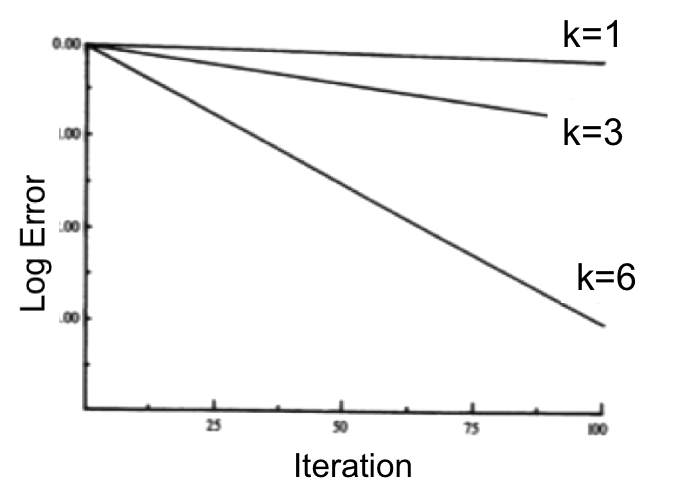
\includegraphics [width=0.5\textwidth, height=0.3\textheight] {FourierError}
   \end{center}
   \caption{Log of Error As a Function of Iteration Count When a Relaxer is Applied to Three Fourier Modes \cite{Briggs2000}}
   \label{fig:FourierError}
\end{figure}
%
The rapid removal of oscillatory and slow removal of coarse error modes is often seen in practice. Figure~\ref{fig:MGerrorExample} shows an error plot that exhibits this behavior
%
\begin{figure}[!ht]
    \begin{center}
      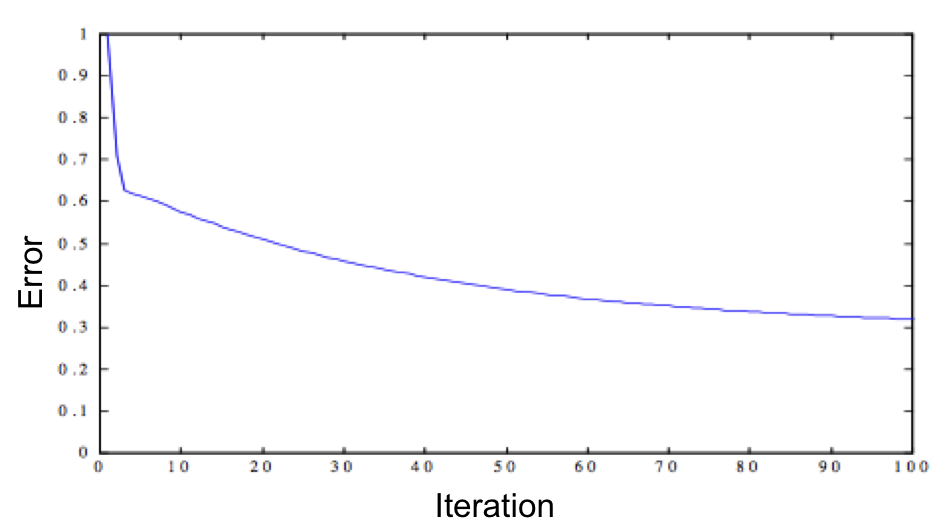
\includegraphics [width=0.7\textwidth, height=0.4\textheight] {MGerrorExample}
   \end{center}
   \caption{Error As a Function of Iteration Count. Oscillatory Components Are Removed Rapidly, Leaving Smooth Components \cite{Briggs2000}}
   \label{fig:MGerrorExample}
\end{figure}

The idea of multigrid methods is to take advantage of the smoothing effect by making smooth error look oscillatory so it can be more easily removed. Error that is low frequency on a fine grid can be mapped onto a coarser grid where it is oscillatory. This change can be thought of as increasing the number of oscillations per grid point. Look at Figure~\ref{fig:FourierGridError} for an example. When $n$ = 12, the maximum number of half-sine waves is 12, so $k$ = 4 is relatively smooth. When mapped to $n$ = 6, $k$ = 4 is relatively oscillatory. 
%
\begin{figure}[!ht]
    \begin{center}
      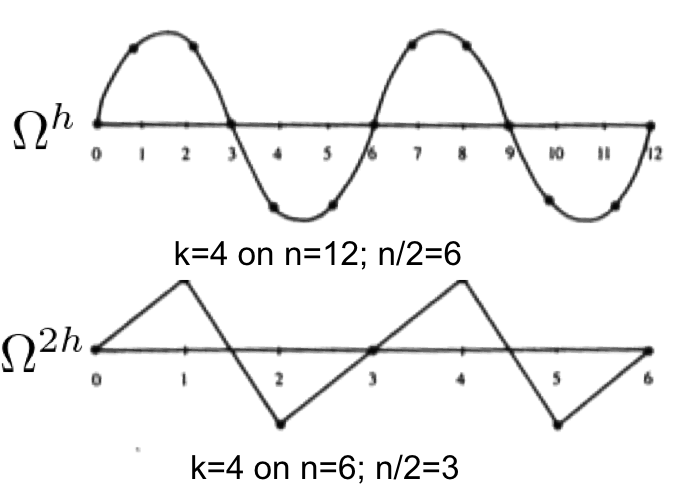
\includegraphics [width=0.55\textwidth, height=0.33\textheight] {FourierGridError}
   \end{center}
   \caption{Relative Oscillation of a Fourier Mode Mapped Between Two Grids \cite{Briggs2000}}
   \label{fig:FourierGridError}
\end{figure}

Using this information, multigrid methods can be understood. The error is mapped from a fine grid to a coarser grid. A smoother is applied on the coarse grid to remove the newly oscillatory error components. The result is mapped back to the fine grid and used to correct the solution there. A few more relaxations are done back on the fine grid. That whole process is called a v-cycle, which is described in Algorithm~\ref{algo:MG}. A call to this method is symbolized as $v^h \leftarrow \ve{G}(v^h, b^h)$ and is effectively doing $v^{h} \approx \ve{G}^{-1}b^{h}$.
%
\begin{algorithm}
  \caption{ Multigrid v-cycle: $v^h \leftarrow \ve{G}(v^h, b^h)$}
  \label{algo:MG}
  \begin{list}{}{\hspace{2.5em}}
    \item Relax $\nu_1$ times on $\ve{A}^h u^h = b^h$ on the fine grid $\Omega^h$ using initial guess $v^h$.
    \item Compute the residual, $r^h = b^h - \ve{A} v^h$. 
    \item Using some restriction operator, $\ve{R}_h^{2h}$, restrict the residual to a coarser grid: $r^{2h} =  \ve{R}_h^{2h} r^h$. 
    \item Solve the residual equation, $\ve{A}^{2h} e^{2h} = r^{2h}$, on coarse grid $\Omega^{2h}$. 
    \item Using some prolongation operator, $\ve{P}_{2h}^h$, prolong (interpolate) the coarse grid error back to a finer grid: $e^h = \ve{P}_{2h}^h e^{2h}$. 
    \item Add the error to the fine grid guess: $v^h \rightarrow v^h + e^h$. 
    \item Relax $\nu_2$ times on $\ve{A}^h u^h = b^h$ on $\Omega^h$ to get an improved solution. 
   \end{list}
\end{algorithm}

The details of how restriction and prolongation are done are problem dependent. Simple iterative schemes can have very simple operators while more complex schemes may require more complex mappings. Other implementation choices are what relaxer to use and how many relaxations to do on each grid.

There are many variations of how multigrid methods are put together. All methods, however, are built on the basic v-cycle correction scheme. A V-cycle is an extension of the v-cycle. Instead of only using two grids, many grids are used. The problem is restricted from grid to grid until it is on some grid which is coarse enough to directly invert the equations. Then the errors are prolongated back up the chain, continuously correcting on finer grids, until the finest grid is reached. Multigrid methods are differentiated by how many times the V-cycle is done and how many grids are used. A five-grid V-cycle can be seen in Figure~\ref{fig:Vcycle} (a). A W-cycle is when V-cycles are repeated to further improve the answer. An example can be seen in Figure~\ref{fig:Vcycle} (b). 
\begin{figure}
    \begin{center}
      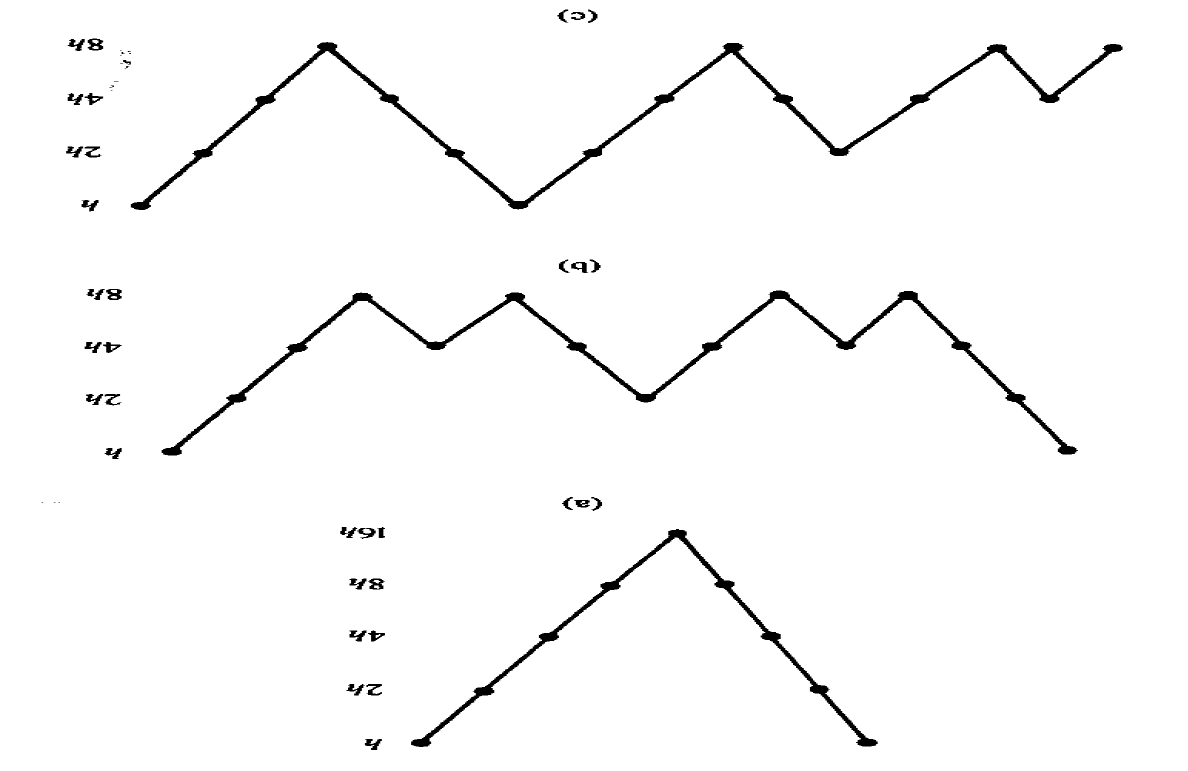
\includegraphics [width=0.7\textwidth, height=0.7\textheight, angle=180 ] {multigridFig}
   \end{center}
   \caption{Grid Schedule for (a) a V-cycle, (b) a W-cycle, and (c) a Full Multigrid Pattern \cite{Briggs2000}}
   \label{fig:Vcycle}
\end{figure}

Multigrid can also be used to obtain an initial guess where much of the smooth error has been removed. This is called nested iteration, and the iterations begin on the coarsest grid and move up to the finest grid. If nested iteration is combined with V-cycles, the full multigrid method (FMG) is obtained, as seen in Figure~\ref{fig:Vcycle} (c). A call to any of the combinations of v-cycles is denoted $v \leftarrow \ve{G}(v, b)$. The optimal combination of grids and cycles may depend on problem type. The addition of more grids and cycles will reduce error, but at an added cost. 

Multigrid methods can be thought of as stationary iterative schemes that can be used alone or as accelerators for other methods. In the past these methods were highly problem specific and only applied to second-order elliptic PDEs. Over time they have been extended to different problem types, geometries, and discretizations \cite{Benzi2002}. 

%-------------------------------------------------------------------------------------------------------
%-------------------------------------------------------------------------------------------------------
\section{Past Work}
This section discusses some past work from most of the categories of preconditioners that were presented above. The focus is on methods that have been used to precondition Krylov solvers and on multigrid methods. This section is intended to illustrate the need for preconditioning Krylov methods in transport and to demonstrate the new preconditioner's originality. 

As an aside, it is important to note that how well a preconditioner is going to do for a certain problem when using Krylov methods cannot be known a priori. At this time there are no set methods or procedures for predicting preconditioner behavior with Krylov methods. As a result, preconditioning Krylov methods is somewhat ``guess and check.'' Despite this, the reward of preconditioning Krylov methods ensure that they are an essential part of their practical use \cite{Knoll2004}, \cite{Benzi2002}. 

%-------------------------------------------------------------------------------------------------------
\subsection{Rebalance}
CMR has been widely used in transport codes since at least the 1970s and new variants of it are being applied to Krylov solvers \cite{Dahmani2002}, \cite{Yamamoto2005}. For example, Dahmani et.\ al.\ investigated using GMRES and preconditioned GMRES for solving the 3-D transport equation using the method of characteristics (MOC) in 2005. Self-collision rebalance (SCR) was used as a left preconditioner. SCR uses the probability of a region scattering particles to itself to rebalance the energy distribution in each region. MOC is quite different from \Sn and requires a specific derivation to be able to use GMRES \cite{Dahmani2002}. 

%-------------------------------------------------------------------------------------------------------
\subsection{Incomplete Factorizations}
Incomplete factorizations have also been used to precondition Krylov methods, though without much success for large transport problems. Patton and Holloway investigated the use of a variety of preconditioners for GMRES to solve the multi-group, diamond-difference, 1-D, \Sn equations. They compared matrix-based and physics-based right preconditioners. A variety of factorization methods, the matix-based preconditioners, were considered: ILU(0), modified ILU(0) (MILU), ILU($\tau=10^{-4}$), ILU($p=10$), and ILU($\tau=10^{-4}, p=10$), where $\tau$ is the drop tolerance and $p$ indicates the amount of fill-in allowed. A single integer indicates the fill-in limit. 

The bandwidth of $\ve{A}$ increases as the number of energy groups and/or discrete ordinates increases \cite{Patton2002}. Here, the bandwidth of the matrix is $2GM$ where $G$ is the number of energy groups and $M$ is the number of discrete ordinates. The computational time required by ILU factorization increases with the bandwidth of $\ve{A}$. This makes factorization methods unattractive as accelerators for finely discretized problems. This prompted Patton and Holloway to consider physics-based methods. 

%A matrix splitting was chosen such that the original problem formulation was written as:
%%
%\begin{equation}
%  \ve{L}\psi - \ve{S}_{in}\psi = \ve{Q} \:,
%\end{equation}
%%
%where $\ve{L}$ is the streaming plus removal term, $\ve{S}_{in}$ is the inscattering source, and $\ve{Q}$ contains the external source. Patton and Holloway use $(\ve{L} - \ve{S}_{down})^{-1}$ as the preconditioner, where  $\ve{S}_{down}$ is the downscatter part of the $\ve{S}$ matrix. They use source iteration as the within-group solver such that each new guess is obtained by applying $(\ve{L} - \ve{S}_{down})^{-1}(\ve{S}_{in} - \ve{S}_{down})$ to the old guess. 
A matrix splitting method was chosen that used physics rather than generic structural properties to inform how to do the splitting. They used source iteration as the within-group solver. For the 1-D case they found that this physics-based preconditioner was faster than the matrix-based factorization preconditioner, but that DSA was faster than both \cite{Patton2002}. This is not surprising for the 1-D case with diamond difference. 

In 2004 Chen and Sheu compared preconditioned conjugate gradient methods with SOR for 3-D, multigroup neutron transport. They used ILU and MILU to precondition both conjugate gradient squared (CGS) and BiCGSTAB. They chose these iterative techniques because they have good residual error control procedures that give good convergence rates in general \cite{Chen2004}.

Kozlowski, Downar, and Lewis investigated a Krylov preconditioning method for the multi-group $SP_3$ transport equations. This method involves reordering the fluxes to facilitate the use of block ILU as the preconditioner. This idea worked well for small problems, but may require too much storage for large problems \cite{Kozlowski2003}.

%-------------------------------------------------------------------------------------------------------
\subsection{Synthetic Acceleration}
DSA has been under continuous development since Alcouffe's 1977 paper. For example, a recent research string began when Wareing, Larsen, and Adams developed a simple DSA scheme for bilinear discontinuous (BLD) discretizations schemes in 2-D. An unconditionally efficient multigrid technique for solving these 2-D, BLD equations was derived by Morel, Dendy, and Wareing. This was later extended to bilinear nodal differencing and bilinear characteristic differencing \cite{Adams2002}. New versions of DSA are applied to Krylov solvers in current transport codes.

Very recently Rosa et.\ al.\ performed detailed Fourier Analysis on TSA combined with Inexact Parallel Block-Jacobi (IPBJ) splitting applied to the one- and two-dimensional transport cases. They noted that both experience in the nuclear community and analytical work have shown that solution methods such as GMRES(m) can stagnate for problems containing optically thin spatial regions. Rosa et.\ al.'s analysis and results show that using modified TSA improves the spectral properties such that convergence can be obtained using a relatively small m when using GMRES(m) \cite{Rosa2010}.

\subsubsection{DSA in Denovo}
Denovo has the option to use DSA to precondition the within-group transport equation, $\bigl(\ve{I} - \ve{DL}^{-1}\ve{MS}_{gg}\bigr) \phi_{g} = \ve{DL}^{-1}Q_{g}$, which works very well when using a Krylov method. High-frequency error modes are what often cause instability in DSA. Krylov iteration, like iterative methods in general, will rapidly damp such oscillatory modes. Eliminating the high-frequency error enables the removal of the consistency requirement since DSA is not likely to fail when those error modes are gone \cite{Evans2009d}. This means DSA can be applied successfully for a variety of spatial discretizations. 

The DSA-preconditioned one-group equation is:
%
\begin{equation}
  \bigl(\ve{I} + \ve{PC}^{-1}\ve{RS}\bigr) \bigl(\ve{I} - \ve{DL}^{-1}\ve{MS}\bigr) \phi = \bigl(\ve{I} + \ve{PC}^{-1}\ve{RS}\bigr)\ve{DL}^{-1}\bar{Q} \:. 
  \label{DSA1group}
\end{equation}
%
Here $\ve{C}$ is the diffusion operator defined in Appendix~\ref{sec:AppendixA}; $\ve{R}$ is the restriction operator, which maps the transport solution onto the diffusion vector; and $\ve{P}$ is the projection operator, which maps the diffusion vector onto the transport solution. Denovo does not actually form these operators, instead it solves the diffusion equation and updates the $\phi_{00}$ moments. In practice this means that for a Krylov iteration
%
\begin{equation}
  \ve{C}z = \ve{RS}\bigl(\ve{I} - \ve{DL}^{-1}\ve{SM}\bigr) v
\end{equation}
%
is solved for each group. In Denovo, DSA has been found to be beneficial for diffusive problems with high scattering ratios that are close to being isotropic \cite{Evans2009d}. This is consistent with experiences of the wider nuclear community.

%-------------------------------------------------------------------------------------------------------
\subsection{Multigrid Methods}
Beginning in the late 1980s, the nuclear community started using spatial \mg and/or angular \mg as both solvers and preconditioners. The first use of spatial \mg for transport equations in 1-D and 2-D was investigated by Nowak et.\ al. Since that time \mg has been used in multiple dimensions, for both isotropic and anisotropic scattering, and for various spatial discretizations \cite{Adams2002}. Some highlights from recent work are discussed below. All are applied to the \Sn neutron transport equation unless otherwise noted. 

In 1996 Sjoden and Haghighat used a simplified spatial \mg method that does not use the residual as a solver for the 3-D, parallel code PENTRAN \cite{Sjoden1996}. In 1998 multigrid in space and multigrid in angle were used as preconditioners for Krylov methods and were tested for the 1-D, one-group, modified linear discontinuous (MLD) neutron transport equations by Oliveira and Deng. They looked at isotropic scattering without absorption, isotropic with absorption, and anisotropic cases. They had better results with multigrid than when using ILU as a preconditioner \cite{Oliveira1998}.

In 2007 Chang et.\ al.\ used 2-D spatial \mg for the isotropic scattering case with corner balance finite difference in space and a four-color block-Jacobi relaxation scheme. A bilinear interpolation operator and its transpose were used for grid transfer. The method had some trouble with heterogeneous problems. The authors assert their algorithm is parallelizable \cite{Chang2007}.

In 2010 Lee developed a method to do \mg in space and angle simultaneously for two and three dimensions, isotropic and anisotropic scattering, one energy group, and a variety of spatial discretizations. The method can perform \mg only space, only angle, or some combination there of. It also handles thick and thin cells \cite{Lee2010}.

This list is hardly comprehensive, but is intended to be representative of new and recent developments in this area. The author was unable to find any cases where \mg was used in the energy variable either as a solution technique or as a preconditioner. 

\subsubsection{Two-Grid Acceleration}
The two-grid acceleration method developed by Adams and Morel was one of the earlier spatial \mg methods and it has been built upon by others \cite{Adams1993}. It is intended to accelerate convergence of the outer iterations for the transport equation when upscattering is present; the outer iteration method is Gauss Seidel. The original work was done for slab geometry with linear discontinuous (LD) discretization, and the method is a one-grid, one-cycle scheme in angle. The general approach is expounded upon here to provide an example of \mg methods applied to the transport equation and because a variation of this method is used in Denovo. 

Adams and Morel create a within group error equation by subtracting the GS equation from the transport equation. If the error in iteration $k$ is $\epsilon^k$ and the $l$th moment of the residual is $R_l^k$, then for group $g$ in 1-D this gives:
%
\begin{align}
   \mu \frac{\partial \epsilon_{g}^{k+1}(\mu)}{\partial x} + \Macro_{t,g} \epsilon_{g}^{k+1}(\mu) &= \sum_{l=0}^{L}\frac{2l+1}{4\pi} \bigl( \sum_{g'=1}^{g}\Macro_{s,g' \to g, l} \epsilon_{g',l}^{k+1} 
   +  \label{eq:GSerror} \\
   &\sum_{g'=g+1}^{G}\Macro_{s,g' \to g, l} \phi_{g',l}^{k} + R_{g,l}\bigr) P_{l}(\mu) \:, \nonumber \\
  \epsilon_{g}^{k+1}(\mu) &= \psi_{g}(\mu) - \psi_{g}^{k+1}(\mu) \:, \\
  \epsilon_{g',l}^{k+1} &= 2\pi \int_{-1}^{1}\epsilon_{g'}^{k+1}(\mu') P_{l}(\mu') d\mu' \:, \\ 
  R_{g,l}^{k+1} &=  \sum_{g'=g+1}^{G}\Macro_{s,g' \to g, l} \bigl( \phi_{g',l}^{k+1} - \Macro_{g',l}^{k} \bigr) \:.
\end{align}
%
The diffusion approximation is applied to Equation \eqref{eq:GSerror}, giving a coarse grid equation. The coarse grid equation is then solved on the coarse grid for the error, which is in turn added to the flux approximation. 

Next, it is assumed that the zeroth moment of the error is a product of a spectral shape function, $\xi_g$ and a space-dependent modulation function, $E(x)$:
%
\begin{align}
  \epsilon_{g,0}^{k+1}(x) &= E(x)\xi_{g} \:, \text{ and} \label{eq:errorExpand} \\
  \sum_{g=1}^{G} \xi_{g} &= 1 \:.
\end{align} 
%
The spectral shape function corresponds to the slowest converging error mode, i.e.\ the mode to be eliminated. To find the shape function, Fourier analysis is performed on the GS iterative method. The zeroth moment of the cross sections is used to form the Fourier matrix, and then an eigenproblem can be formed. The spectral radius of the isotropic GS matrix is the eigenvalue, and the corresponding eigenvector is the shape function. Because the shape function is dependent on materials, one such calculation must be done for each material region. Note that by using the zeroth moment only the isotropic component of the solution is accelerated.

The coarse grid diffusion equations that result from Equations \eqref{eq:GSerror} and \eqref{eq:errorExpand} differ slightly in form from the standard diffusion equation in that there is an extra term containing the gradient of the shape function. This is zero in homogeneous regions, but undefined at material interfaces. Adams and Morel found that neglecting the gradient term all together still gave good results for their test problems. This may not be true for more complex cases.

The two-grid method requires the diffusion operator to be consistent with the transport operator, just like in DSA. This requirement can be difficult to meet for multi-dimensional problems, particularly for some spatial discretizations. 

\subsubsection{Two-Grid in Denovo}
\label{sec:TTG}
Denovo has a two-grid acceleration scheme based on the one developed by Adams and Morel. As noted above, the iteration procedure uses a collapsed one-group diffusion equation to correct the low-order Fourier modes \cite{Adams1993}. Because of the consistency requirement for the discretization of the diffusion operator in multi-dimensional and multi-material problems, this method can fail for systems of interest \cite{Evans2009d}. 

The original two-grid method was modified by Evans et.\ al.\ to make it applicable for the desired cases by using a one-group transport equation instead of the diffusion equation. The modified method is called transport two-grid (TTG). Adams and Morel showed that the slowest converging spatial modes are diffusive and can be exactly computed in the infinite homogeneous case. To preserve this, the TTG method gives the correct error estimation in that limit \cite{Evans2009d}. 

The cross sections used in TTG are therefore calculated to give the same energy-collapsed cross sections as the diffusion equation for the infinite homogeneous case, as seen in Equations \eqref{TTGxsecs1} and \eqref{TTGxsecs2}. TTG solves a one-group transport equation for the low-order error in each GS iteration, where $[g1, g2]$ is the group range of the upscatter block:
%
\begin{align}
  \ve{\hat{\Omega}} \cdot \nabla \psi_{\epsilon} &+ \bar{\Macro}\psi_{\epsilon} = \frac{1}{4\pi}\bar{\Macro}_{s}\phi_{\epsilon} + \frac{1}{4\pi}\bar{R} \:, \\
  \bar{\Macro} &= \frac{1}{\sum_{g=g_1}^{g_2} \frac{1}{\Macro^g}\zeta^g} \label{TTGxsecs1} \:,\\
  \bar{\Macro}_{s} &= \frac{1}{\sum_{g=g_1}^{g_2} \frac{1}{\Macro^g}\zeta^g} - \sum_{g=g_1}^{g_2} \bigl(\Macro^g\zeta^g - \sum_{g'=g_1}^{g_2} \Macro_{s0}^{gg'} \zeta^{g'} \bigr) \label{TTGxsecs2} \:. 
\end{align}
%
The spatial components of the error are $\psi_{\epsilon}$ and $\phi_{\epsilon}$; $\bar{R}$ is the residual. Just as in the original method, it is assumed that the error is separable in space and energy at each iteration: $\epsilon_g^k = \phi_g - \phi_g^k = \phi_{\epsilon}(\vec{r})\zeta^g$, where $\zeta^g$ is a material-dependent spectral function \cite{Evans2009d}. 

To execute the TTG scheme in Denovo, a transport sweep in conducted in each group, a residual is calculated, the low-order transport solve described above is performed, an error form of the transport sweep is conducted, and the scalar flux is updated. All of that can be seen in the following equations: 
\begin{align}
  \ve{L}_g \psi_g^{k+\frac{1}{2}} &= \ve{M}\bigl(\ve{S}_{gg}\phi_g^{k+\frac{1}{2}} + \sum_{g'=g_1}^{g-1} \ve{S}_{gg'}\phi_{g'}^{k+\frac{1}{2}} + \sum_{g'=g+1}^{g_2}\ve{S}_{gg'}\phi_{g'}^k \bigr) + q_{e,g}  \:, \\
  R^{k+\frac{1}{2}}_g &= \ve{M} \sum_{g'=g+1}^{g_2}\ve{S}_{gg'} \bigl( \phi_{g'}^{k+\frac{1}{2}} - \phi_{g'}^k \bigr) \:, \qquad l = m = 0 \:, \\
  \bar{\ve{L}}\psi_{\epsilon} &= \ve{M\bar{S}} \phi_{\epsilon} + \bar{R} \:, \qquad l = m = 0 \:, \label{TTGerrorEqn} \\
  \phi_g^{k+1} &= \phi_{g}^{k+\frac{1}{2}} + \phi_{\epsilon}\zeta^g \:, \qquad l = m = 0 \:.
\end{align}
The operators with over-bars use the collapsed cross sections given in Equations \eqref{TTGxsecs1} and \eqref{TTGxsecs2}, and $\bar{R} = \sum_{g=g_1}^{g_2} R_g^{k+\frac{1}{2}}$. 

The $\zeta_g$ term is calculated from the eigenvalue problem obtained through Fourier analysis of the GS method using isotropic scattering, just like the original two-grid method:
%
\begin{equation}
  \bigl(\ve{T}_{\Macro} - \ve{S}_L + \ve{S}_D\bigr)^{-1} \ve{S}_U\zeta = \rho\zeta \:,
\end{equation}
where $\ve{T}_{\Macro}$ is the diagonal, total cross section matrix. As with the original two-grid method, the TTG method is limited to correcting only the isotropic flux moments. This is an adequate limitation as these moments are dominant in thermal groups where upscattering is most prevalent\cite{Evans2009d}.   

The additional cost of the method is like solving one extra group, so for cases with many upscattering groups the cost can be amortized. The acceleration equation can be preconditioned with DSA for additional speed. Finally, a reduced quadrature set can be used when solving Equation~\eqref{TTGerrorEqn} to limit the cost. Some test problems have shown TTG to be quite effective in improving the speed of convergence for upscatter problems when compared to unaccelerated GS \cite{Evans2009d}.

%-------------------------------------------------------------------------------------------------------
Clearly, a wide variety of preconditioning techniques have been applied to the neutron transport equation. It is worth noting that many of these methods are dependent upon the choice of spatial discretization employed, only apply to within group iterations, or have other important limitations. Preconditioning Krylov methods for solving the neutron transport problem is an active and vital area of research where much progress has been made and in which there is still much room for development. 

%-------------------------------------------------------------------------------------------------------
%-------------------------------------------------------------------------------------------------------
\section{Multigrid in Energy}
Preconditioning is a very important part of increasing the robustness of Krylov methods. This is particularly true in this work for two reasons. The first is that the multigroup Krylov solver can create very large Krylov subspaces because it forms the subspaces with multiple-group-sized vectors. As a result, any reduction in iteration count will have a large benefit in terms of both memory and cost per iteration. The second is that preconditioning is needed to compensate for the ill-conditioned systems created by RQI so that the eigenvector can be converged. 

A new physics-based preconditioner has been added to Denovo to improve the performance of the Krylov solves. It does multigrid in energy. Choosing a physics-based preconditioner supports the goal of accelerating a code that solves a specific equation, not developing an all purpose preconditioner. It makes sense to take advantage of information specific to the neutron transport equations. The past work section showed physics-based preconditioners often provide more benefit than matrix-based methods. Further, the matrix $\ve{A}$ is never formed in Denovo, making matrix-based preconditioners impossible. 

The concept of multigrid in energy is that the grid is in energy, not space or angle like methods used in other work. There are two pieces to this choice, the multigrid piece and the in energy piece. The selection of multigrid is based on the fact that multigrid methods have been successful at accelerating the transport equation and that the convergence behavior of the Krylov iterations inside RQI looks like a very good candidate for multigrid methods. 

The selection of using grids in energy rather than space or angle is to make a preconditioner that can easily take advantage of energy parallelization. The preconditioner works with the MG Krylov method. Having grids in energy means that each energy set can work on its own grids without communicating with other sets. An additional benefit is the simplicity of energy grids. Energy is only one dimension, which makes the grids much less complex (and likely less costly) than angular or multi-D spatial grids. 

%-------------------------------------------------------------------------------------------------------
\subsection{Method}
To make energy grids, the energy group structure is coarsened so each lower grid has fewer groups on it. The finest grid is the input energy structure, and the coarsest grid has one or a few groups. Each level has half as many groups as the previous level, rounded up if applicable. This is conceptually straightforward because the equations are only one-dimensional in energy and energy groups can be combined (restricted) and separated (prolonged) linearly. 

The implemented restriction operator is a simple averaging scheme. Neighboring fine data are averaged together to make coarse data. Recall that for a grid with spacing $h$, $2h$ is the next-coarser grid. The moments are restricted as $\phi_{g}^{2h} = \frac{1}{2}(\phi_{2g}^{h} + \phi_{2g+1}^{h})$ for $g = 1,...,G$, where $G$ is the number of groups on coarse grid and $2G+1$ is the number of groups on the fine grid. If there are an odd number of groups the lowest energy group is just copied. This scheme was chosen so that the thermal energy groups would retain more granularity, which should improve accuracy for thermal reactors. The moments are restricted every time there is transfer to a coarser grid.

The cross sections are restricted from the finest to the coarsest grid during problem initialization and they do not change thereafter. The total and fission cross sections are restricted in the same way as the moments. Scattering is slightly more complicated since it is in two dimensions, $g$ and $g'$. When there are an even number of groups all cross sections are treated the same way. For $g' = 1,..., G'$ and $g = 1, ..., G$,
\begin{equation}
  \Sigma_s^{2h}(g,g') = \frac{1}{4}[\Sigma_s^{h}(2g,2g') + \Sigma_s^{h}(2g+1,2g') + \Sigma_s^{h}(2g,2g'+1) + \Sigma_s^{h}(2g+1,2g'+1)] \:. 
  \label{eq:XSSeven}
\end{equation}
% 
Unless there is upscattering in every group, some of the entries in Equation~\eqref{eq:XSSeven} will be zero. When there are an odd number of groups Equation \eqref{eq:XSSeven} is used until $g=G-1$ and $g'=G'-1$. For the last group
  \begin{align}
    \Sigma^{2h}_s(G,g') &= \frac{1}{2}[\Sigma^{h}_s(2G,2g') + \Sigma^{h}_s(2G,2g'+1)] \qquad \text{for } g' = 0,...,G'-1 \:,\nonumber \\
    \Sigma^{2h}_s(g,G') &=  \frac{1}{2}[\Sigma^{h}_s(2g,2G') + \Sigma^{h}_s(2g_1,2G')] \qquad \text{for } g  = 0,...,G-1 \:,\nonumber \\
    \Sigma^{2h}_s(G,G') &= \Sigma^{h}_s(2G,2G') \nonumber \:.
  \end{align}

To prolong from a coarse grid to a fine, the points that line up between the grids are mapped directly: $\phi_{2g}^{h} = \phi_{g}^{2h}$. To fill in the intermediate points on the fine grid, the adjacent coarse values are linearly interpolated: $\phi_{2g+1}^{h} = \frac{1}{2}(\phi_{g}^{2h} + \phi_{g+1}^{2h})$. The moments are prolonged every time there is a transfer to a finer grid. Since cross sections do not change they are never prolonged. 

The choice of how to restrict and prolong between grids is hard-coded into the preconditioner. There are other multigrid method choices that are easier to vary and some of these are taken as user inputs. The number of V-cycles is a user input. One V-cycle goes from the finest grid to the coarsest grid and back up, but the user can choose to do more than one V-cycle per application. That means that for one application of the preconditioner ($v \leftarrow \ve{G}(v,b)$), any number of the large Vs seen in Figure~\ref{fig:Vcycle} (a) are concatenated together. One cycle looks like one V, two cycles looks like one W, and so on. The default number of V-cycles is 2. The idea is that each additional V-cycle will remove more error. 

At this time the depth of the V-cycle is prescribed by the number of groups. This is set such that the grids will be coarsened until there is only one energy group. The number of grids needed is given by \cite{BinaryTree2011}
\begin{equation}
  \text{floor}\bigl( \frac{ln(G-1)}{ln(2)}\bigr) + 2 \:.
  \label{eq:NumGrids}
\end{equation}
%
This is handled differently with energy sets, as discussed below. The depth of the cycle is an option that could be changed in the future if it is found that restricting down to only one group is unnecessary, particularly if there are a large number of groups. Investigating the optimal V-cycle depth is an important issue, but beyond the scope of this work. 

Some number of relaxations are performed on each grid that makes up a V-cycle. The number of relaxations per level, $\nu_{1,2}$ from Algorithm~\ref{algo:MG}, is a user input choice with a default of 2. Doing more relaxations per grid should remove more error overall. The implemented relaxation method is weighted Richardson iteration, whose $k$th step is
%
\begin{equation}
  \phi^{k} = \phi^{k-1} + \omega^{k}\ve{P}^{-1}(b^{k-1} - \ve{A}\phi^{k-1}) \:.
  \label{eq:Richardson}
\end{equation}
%
$\ve{P}$ is some easily invertible matrix, the details of which determine exactly what method is being used. If $\omega^{k}$ is constant then this is the stationary Richardson method \cite{Moore1999}. 

In this work $\ve{P} = \ve{I}$ and $\ve{P}^{-1} = \ve{I}$, and $\omega$ is a constant and selected by the user that defaults to 1. When applied to the Transport equation, this looks like
%
\begin{align}
  \phi^{k} &= \phi^{k-1} + \omega\bigr(b^{k-1} - (\ve{I} - \ve{TMS})\phi^{k-1}\bigl) \:, \text{ or} \nonumber \\
  \phi^{k} &= \bigr(\ve{I} + \omega(\ve{TMS} - \ve{I})\bigl)\phi^{k-1} + \omega b^{k-1} \:.
  \label{eq:relax}
 \end{align}
  
An important principle is that the preconditioner is only attempting to roughly invert $\ve{A}$, so choosing to simplify the solver beyond the method alone, i.e.\ Richardson instead of Krylov, is reasonable. In this vein there is an option to use a smaller angle set in the preconditioner than the rest of the solution. For example, the whole problem can be solved at $S_{10}$, but the preconditioner would only use $S_{2}$. There is an input option to specify what to use in preconditioner; the default is whatever is being used by the entire problem. This is only available for problems with vacuum boundary conditions at this time. 

Recall that right preconditioning is applied as $\ve{A} \ve{G}^{-1} \ve{G} \phi = b$, where $\ve{A} = \ve{I} - \ve{TMS}$. To implement this in Denovo, the problem must be broken up into several steps: 
%
\begin{align}
  \text{Define} \qquad y &= \ve{G}\phi \:;\\
  \text{with a Krylov method solve} \qquad \ve{AG}^{-1}y &= b \:. \\
  \text{After finding }y\text{, the final step is} \qquad \phi &= \ve{G}^{-1}y \:.
\end{align}
%
The Krylov solvers cannot be modified easily because they are provided by an external library, so carrying out the second step means the preconditioner must be applied to the iteration vectors handed to the solver. Equations~\eqref{eq:invertG}, \eqref{eq:ApplyA}, and \eqref{eq:findPhi} show how this works.  

Let $v^{j}$ be an iteration vector that represents $y$, and let $z^{j}$ be an intermediate iteration vector. At each step below the equations are shown three ways to make clear what is going on algorithmically: the equation being solved, the symbolic representation of the outcome, and the way this is written in multigrid syntax. The first thing is to apply the preconditioner to the intermediate vector: %to affect the inversion of $\ve{G}$,
%
\begin{align}
  \ve{G}z^{j} &= v^{j} \:,  \label{eq:invertG} \\
  z^{j} &\approx \ve{G}^{-1}v^{j} \:, \nonumber \\
  z^{j} &\leftarrow \ve{G}(z^{j}, v^{j}) \:. \nonumber
\end{align}
%
Next, apply $\ve{A}$ to $z^{j}$ and set it equal to $v^{j+1}$:
\begin{align}
  v^{j+1} &= \ve{A}z^{j} \:,   \label{eq:ApplyA} \\
  v^{j+1} &\approx \ve{AG}^{-1}v^{j} \:, \nonumber \\
  y = v^{j+1} &= \ve{A}[z^{j} \leftarrow \ve{G}(z^{j}, v^{j})] \:. \nonumber
\end{align}
%
To get the final $\phi$ from $y = \ve{G}\phi$, apply the preconditioner again to an iteration vector $w$ and $\phi = w^{j}$:
%
\begin{align}
  \ve{G}w^{j} &= y \:,   \label{eq:findPhi} \\
  w^{j} &\approx \ve{G}^{-1}y \:, \nonumber \\
  \phi = w^{j} &\leftarrow \ve{G}(w^{j}, y) \:. \nonumber
\end{align}

The operator is used within the preconditioner to compute the residual, $r = \ve{A}\phi - b$, and the form of the operator is used in the relaxation method. The default behavior when doing RQI is to use the regular, unshifted operator in the preconditioner. There is an option to use the shifted operator instead. In that case $\mathbf{S}$ becomes $\tilde{\ve{S}} = \ve{S} + \rho\ve{F}$ and the right hand side becomes $(\frac{1}{k} - \rho)\ve{TMF}\phi$. The use of the shifted operator can be turned on through an input option. This changes the calculation of the residual as well as the $\ve{S}$ used in the relaxer.

An important attribute of this preconditioner is that it is parallelizable in energy because it can use the energy sets introduced earlier in this work. There are two ways to handle energy grids and energy sets together. One way is to restrict from $G$ groups down to $1$ group just as if there were no energy sets. This requires cross-set communication as soon as there are fewer groups than sets. This also causes some logistical difficulties related to what data is held by which sets at various points in the calculation. 

The other way is to prohibit cross-set communication by having each set do its own ``mini'' V-cycle. Each set restricts, prolongs, and relaxes on only its groups. Instead of restricting to one group overall, each set restricts to one or two group(s), giving approximately num\_sets groups overall. This strategy requires there be at least two groups on every set. The number of grids needed is determined by the set with the minimum number of groups since it will be the first to reach a grid with one group. To choose the number of levels, Algorithm~\ref{algo:multisetsGrids} is used. 
%
\begin{algorithm}
  \caption{ Calculating the Number of Preconditioner Grids When There Are Energy Sets}
  \label{algo:multisetsGrids}
   num\_groups = $G$, num\_levels = 1, num\_local\_min = floor$\bigl( \frac{\text{num\_groups}}{\text{num\_sets}}\bigr)$ \\
   while (num\_local\_min $>$ 1)
  \begin{list}{}{\hspace{2.5em}}
    \item num\_levels = num\_levels + 1
    \item num\_groups = (num\_groups + 1) / 2
    \item num\_local\_min = floor$\bigl( \frac{\text{num\_groups}}{\text{num\_sets}}\bigr)$
   \end{list}
\end{algorithm}

The communication costs and logistical complications of the first strategy seem likely to overwhelm the benefit gained by going to one group instead of num\_sets groups. The second strategy was chosen because it involves much less communication and overhead cost. The validity of this choice will be commented upon in the results section. 

With the implemented energy set strategy there are tradeoffs between the number of sets and number of grids for a fixed number of groups. When there are more sets, more cores can be used at one time and wall time should decrease. When there are fewer sets each V-cycle can go deeper so the preconditioner should be more effective, which will reduce iteration count and hopefully decrease wall time. This tradeoff is also investigated.

%-------------------------------------------------------------------------------------------------------
\subsection{Results}
Fully characterizing the behavior of the preconditioner is not simple because there are so many variables. The variety of knobs to turn are grouped into three categories: 1) problem and solver type, 2) preconditioning parameters, 3) number of groups and sets. The problem types and solvers are fixed source, eigenvalue with power iteration, and eigenvalue with Rayleigh quotient iteration. All were solved with the multigroup Krylov solver unless otherwise noted. 

The preconditioning parameters are weight, number of V-cycles, and number of relaxations per level. The syntax used throughout this section will be $w\#$ is the weight, $r\#$ is the number of relaxations per level, and $v\#$ is the number of V-cycles, e.g.\ $w1r1v1$ is one relaxation per level, one V-cycle, and a weight of 1. ``More'' or a ``large amount of'' preconditioning means larger values of $w$ and/or $r$ and/or $v$. The group consideration deals with whether there are many or few groups and how many groups per set were used when doing multisets. Calculations were done to investigate as much of the problem space as possible.

In all tests the number of Krylov iterations over the whole calculation are compared. These subspaces are over all groups unless otherwise noted. Some problems report timing as well. Timing comparisons of most problems should be considered somewhat heuristically. In cases where the calculations were done on a single core, the machine was not dedicated to these calculations and times could vary if the same calculations were repeated. Further, little effort has been put into optimizing the preconditioner for speed. Once the multigrid in energy solver has been optimized for efficiency, the preconditioned times should decrease. How much improvement can be gained is a matter for future study. 

\subsubsection{RQI Parameter Scoping}
The first two problems run with the preconditioner were the small Rayleigh quotient iteration unit tests reported on in Chapter~\ref{sec:Chp3}. These easy problems were done to find out three things. The first was to check that the preconditioner reduces the number of Krylov iterations used in an RQI calculation. The second was to get some guidance on the effect of the preconditioning parameters. The third was find out whether or not the shifted version of the operator should be used in the preconditioner. All tests were run on one processor using the debug version of Denovo with GMRES as the multigroup Krylov solver.

The small RQI unit test with vacuum boundary conditions was tested first. In all cases the correct $k$ and flux were found, and the preconditioned version used fewer Krylov iterations than the base case. The number of RQ iterations was not affected by the preconditioning. The tolerance used to compare the flux to the reference case was $1 \times 10^{-5}$. The results are shown in Table~\ref{table:RQIUnitTestVac}.
%
\begin{table}[!h]
\caption{RQI Unit Test With Vacuum Boundaries, Preconditioning Parameter Study}
\begin{center}
\begin{tabular}{c c c c c}
\hline
Weight & Relaxations & V-cycles & Krylov & RQI \\[0.5ex]
\hline
0    & 0 & 0 & 39 & 6 \\
1    & 1 & 1 & 27 & 6 \\
1.2 & 1 & 1 & 31 & 6 \\
1    & 2 & 1 & 16 & 6 \\
1.2 & 2 & 1 & 19 & 6 \\
1    & 1 & 2 & 16 & 6 \\
1.2 & 1 & 2 & 19 & 6 \\
1    & 2 & 2 & 11 & 6 \\
1.2 & 2 & 2 & 11 & 6 \\
\hline
1    & 2 & 3 & 10 & 6 \\
1.2 & 2 & 3 & 10 & 6 \\
1.3 & 2 & 3 & 10 & 6 \\
1.4 & 2 & 3 & 10 & 6 \\
\hline
1    & 3 & 3 & 6   & 6 \\
1    & 4 & 4 & 6   & 6 \\
1.3 & 4 & 4 & 6   & 6 \\
1    & 5 & 5 & 6   & 6 \\
1.3 & 5 & 5 & 6   & 6 \\
\hline 
\end{tabular}
\end{center}
\label{table:RQIUnitTestVac}
\end{table}

To get much benefit from preconditioning this problem, larger values for the $r$ and $v$ parameters were needed. With $w1r1v1$ the Kyrlov iteration count was only reduced from 39 to 27; with $w1r3v3$ it went to 6. When only a small amount of preconditioning is used ($r1v1$), increasing the weight actually increases the number of Krylov iterations needed. When $r$ and $v$ are larger, changing the weight has no effect for this problem. When large values are used for the preconditioning parameters, the problem does not break down. 

Increasing $r$ or $v$ or both reduces the number of Krylov iterations, with an limit of 1 Krylov iteration per Rayleigh quotient iteration. For this problem the effect of $r$ and $v$ on iteration count are the same. That is $r1v2$ gives the same result as $r2v1$. This is not a surprising finding because both of those combinations result in the same number of relaxations being done on the flux moments on each energy grid.

%-------------------------------------------------------------------------------------------------------
This test was also tried with the shifted version of the operator in the preconditioner. Unless otherwise noted the correct $k$ and flux were found. The flux checking tolerance was again $1 \times 10^{-5}$. The results are shown in Table~\ref{table:RQIUnitTestVacShifted}.
%
\begin{table}[!h]
\caption{RQI Unit Test With Vacuum Boundaries and Shifted Operator, Preconditioning Parameter Study}
\begin{center}
\begin{tabular}{c c c c c}
\hline
Weight & Relaxations & V-cycles & Krylov & RQI \\[0.5ex]
\hline
0    & 0 & 0 & 39 & 6 \\
1    & 1 & 1 & 20 & 6$^{*}$ \\
1.2 & 1 & 1 & 31 & 7$^{\dagger}$ \\
1    & 2 & 1 & 12 & 6 \\
1.2 & 2 & 1 & 16 & 6 \\
1    & 1 & 2 & 12 & 6 \\
1.2 & 1 & 2 & 16 & 6 \\
1    & 2 & 2 & 10 & 6 \\
1.2 & 2 & 2 & 10 & 6 \\
1    & 2 & 3 & 6   & 6 \\
\hline 
\end{tabular}\\
$^{*}$flux was not correct and $k$ was 0.17632 instead of 0.17528 \\
 $^{\dagger}$flux was not correct and $k$ was 0.17494 instead of 0.17528
\end{center}
\label{table:RQIUnitTestVacShifted}
\end{table}

Fewer Krylov iterations were needed with the shifted operator than with the unshifted operator. For example, using $w1r2v3$ yielded 6 iterations while the same parameters in the unshifted version yielded 10. However, the two $r1v1$ cases did not get quite the right eigenvalue, suggesting the shifted operator may not be as robust as the unshifted version. Note that this problem occurred when preconditioning values were small. This study demonstrated the same patterns for weight, number of relaxations per level, and number of V-cycles as the unshifted study. 

%-------------------------------------------------------------------------------------------------------
The next test was the small RQI unit test with reflecting boundary conditions. The flux was not tested against a very tight tolerance, either $1 \times 10^{-2}$ or $1 \times 10^{-3}$ unless otherwise noted. Unless the calculation failed, the correct eigenvalue-vector pair were found. The results are shown in Table~\ref{table:RQIUnitTestRefl}. Note that here the maximum number of Krylov iterations was set to 100.
%
\begin{table}[!h]
\caption{RQI Unit Test With Reflecting Boundaries, Preconditioning Parameter Study}
\begin{center}
\begin{tabular}{c c c c c c}
\hline
Weight & Relaxations & V-cycles & $k$ & Krylov & RQI \\[0.5ex]
\hline
0    & 0 & 0 & 2 & 35   & 5 \\
1    & 1 & 1 & 2 & 30   & 2$^{*}$ \\
1.2 & 1 & 1 & 2 & 127 & 2$^{*}$$^{\dagger}$ \\
1.3 & 1 & 1 & 2 & 200 & 2$^{\dagger}$ \\
1.4 & 1 & 1 & 1.9977  & n/a & test failed \\
\hline
0.7 & 2 & 2 & 2 & 13   & 2 \\
0.9 & 2 & 2 & 2 & 12   & 2 \\
1    & 2 & 2 & 2 & 12   & 2 \\
1.2 & 2 & 2 & 2 & 29   & 2 \\
\hline
1    & 3 & 3 & 2 & 8     & 2 \\
1    & 4 & 4 & 2 & 6     & 2 \\
1    & 5 & 5 & 2 & 4     & 2$^{*}$ \\
1.2 & 5 & 5 & 2 & 14   & 2 \\
\hline
1    & 4 & 1 & 2 & 12   & 2 \\
1    & 1 & 4 & 2 & 12   & 2 \\
1    & 4 & 2 & 2 & 8     & 2 \\
1    & 2 & 4 & 2 & 8     & 2 \\
1    & 4 & 3 & 2 & 6     & 2 \\
1    & 3 & 4 & 2 & 6     & 2 \\
\hline 
\end{tabular}\\
$^{*}$used a tighter comparison tolerance of $1 \times 10^{-5}$ and still passed\\
$^{\dagger}$at least one eigenvector iteration did not converge
\end{center}
\label{table:RQIUnitTestRefl}
\end{table}

For this test, the number of RQ iterations were reduced when preconditioning was used, and the number of  Krylov iterations were reduced as long as the eigenvector converged. This problem was more sensitive to increasing the weight than the vacuum problem was. There were no cases in which increasing weight reduced iteration count. With $r1v1$, increasing the weight kept the problem from converging. 

Again, when $r$ and $v$ were increased iteration count went down noticeably. This calculation also showed that exchanging the values of $r$ and $v$ gave the same iteration count. High $r$ and $v$ values reduced iteration count and did not cause breakdown. 

%-------------------------------------------------------------------------------------------------------
The reflecting boundary test was repeated with the shifted version of the operator in the preconditioner as well. Many of these calculations did not pass the unit tests. The flux was tested against the same loose tolerance as the unshifted case unless otherwise noted. The results are show in Table~\ref{table:RQIUnitTestReflShifted}. The maximum number of Krylov iterations was 100.
%
\begin{table}[!h]
\caption{RQI Unit Test With Reflecting Boundaries and Shifted Operator, Preconditioning Parameter Study}
\begin{center}
\begin{tabular}{c c c l c c}
\hline
Weight & Relaxations & V-cycles & $k$ & Krylov & RQI \\[0.5ex]
\hline
0    & 0 & 0 & 2 & 35 & 2 \\
1    & 1 & 1 & test failed \\
1.4 & 1 & 1 & test failed \\
1    & 2 & 2 & test failed \\
1.4 & 2 & 2 & test failed \\
1    & 3 & 3 & test failed \\
1.4 & 3 & 3 & test failed \\
1    & 4 & 1 & test failed \\
1    & 4 & 2 & test failed \\
1    & 4 & 3 & test failed \\
1    & 4 & 4 & 2 & 18 & 6 \\ 
1    & 3 & 4 & test failed \\
1.2 & 3 & 4 & 2.0024 & 41 & 6 \\
1.3 & 3 & 4 & 1.9997 & 1200 & 12 \\
1.4 & 3 & 4 & 2.0037 & 4100 & 41 \\
1    & 5 & 5 & 2 & 8 & 4$^{*}$ \\
1.2 & 5 & 5 & 2& 32 & 4 \\
\hline 
\end{tabular}\\
$^{*}$used a tighter comparison tolerance of $1 \times 10^{-5}$ and still passed
\end{center}
\label{table:RQIUnitTestReflShifted}
\end{table}

This problem only managed to pass and get the right answer with a lot of preconditioning, and only with a few sets of parameters. When the problem did not fail, increasing the weight made the behavior worse. When the problem did not fail, more RQ iterations were taken than without preconditioning, though in 3 cases fewer Krylov iterations were needed. Overall the shifted operator did not work well at all for this problem.

Some preliminary conclusions were drawn from these tests that were used to steer subsequent investigation. A major finding is that using the shifted operator is not useful in the reflecting case, and likely not worth the risk in the vacuum case. With reflecting boundaries the shifted operator nearly always failed. And, while it reduces the number of iterations needed for the vacuum tests, that was only true if ``enough'' preconditioning was used to converge the problem. It is hard to know for sure that sufficient preconditioning was done to get the correct answer. That is, with the shifted operator in the preconditioner the wrong answer might be found and there is no warning that this has happened. 

It is not so surprising that the shifted operator can be troublesome in the preconditioner. Using an ill-conditioned system inside a preconditioner designed to mitigate the effects of ill-conditioning does not make much sense. Just as in the unpreconditioned RQI results, when the shift works it works very well, but most of the time it does not converge. The shifted operator was not investigated further in this work.

With the unshifted operator, the correct $k$ and flux were always found as long as the problem converged. The preconditioner also reduced the number of Krylov iterations as long as the problem converged the eigenvector. In the vacuum case, preconditioning did not reduce the number of RQ iterations, but it did in the reflecting case. 

With vacuum boundary conditions, increasing the weight in the relaxation method was beneficial when larger $r$ and/or $v$ were used. With small $r$ and/or $v$ higher weight was detrimental. A larger $w$ was never useful in the reflecting case. In all cases increasing $r$ and/or $v$ decreased the number of Krylov iterations. The effect of increasing $r$ and $v$ were found to be interchangeable from a Krylov reduction standpoint. 

%-------------------------------------------------------------------------------------------------------
\subsubsection{Fixed Source Parameter Studies}
Using the initial information about the effect of preconditioning parameters gained for the RQI tests, some fixed source tests were done. These are particularly useful because the preconditioner can be studied apart from eigenvalue iterations. All tests were run on one processor using the debug version of Denovo with GMRES as the multigroup Krylov solver.

The first test was a small vacuum boundary test. It used 1 material, 10 groups, 5 upscattering groups, $P_{0}$, $S_{4}$, a 3 $\times$ 3 $\times$ 3 grid, and a tolerance and upscatter tolerance of 1 $\times$ 10$^{-6}$. The first 3 groups had an isotropic source. This problem was used to further study the effects of weight, relaxations per level, and V-cycles.

In one set of tests the weight was varied with the relaxations per level and number of V-cycles both set to 1. The results can be seen in the top plot in Figure~\ref{fig:FxdSrcVac}. It is clear that increasing the weight is initially beneficial, reducing the iteration count to 6 from the unpreconditioned 10. After a certain level, though increased weight begins to increase the number of iterations. A weight of 2 seems to be a ``sweet spot'' that reduced the number of iterations again, though only to 7. However, when a weight of 2.1 was used the problem did not converge. All of the data for the weight study can be found in Appendix~\ref{sec:AppendixD} in Figure~\ref{table:FxdSrcTstVacWeight}.
%
\begin{figure}[!ht]
    \begin{center}
      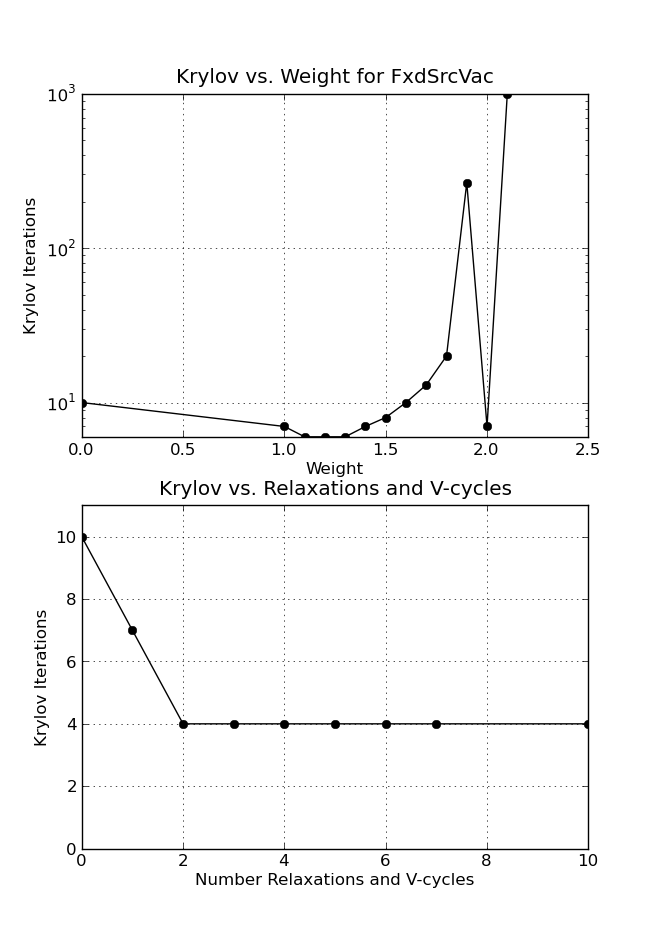
\includegraphics [width=0.7\textwidth, height=0.8\textheight] {FxdSrcVac}
   \end{center}
   \caption{Small Fixed Source Problem with Vacuum Boundaries, Preconditioning Parameter Studies}
   \label{fig:FxdSrcVac}
\end{figure}

Next the number of relaxations per grid and the number of V-cycles were varied with the weight fixed at 1. These results are shown in the bottom plot of Figure~\ref{fig:FxdSrcVac}. Here $r$ and $v$ were changed together, so the number on the x-axis represents both parameters. Initially, increasing $r$ and $v$ reduces the number of iterations needed for convergence. Once the problem gets to 4 iterations no additional amount of preconditioning reduces the iteration count further. The data from this plot is in Appendix~\ref{sec:AppendixD}, Figure~\ref{table:FxdSrcTstVacRV}. A calculation using $w1.3r10v10$ also yielded 4 iterations.

%-------------------------------------------------------------------------------------------------------
The previous problem was repeated with reflecting boundary conditions and two similar studies were done. This time the tolerance and upscatter tolerance were 1 $\times$ 10$^{-6}$. A plot of results for varying the weight with 1 relaxation per level and 1 V-cycle is in the top plot of Figure~\ref{fig:FxdSrcRefl}. The results for varying with number of relaxations per grid and the number of V-cycles with the weight fixed at 1 and some with the weight fixed at 1.3 can be seen in the bottom plot. 
%
\begin{figure}[!ht]
    \begin{center}
      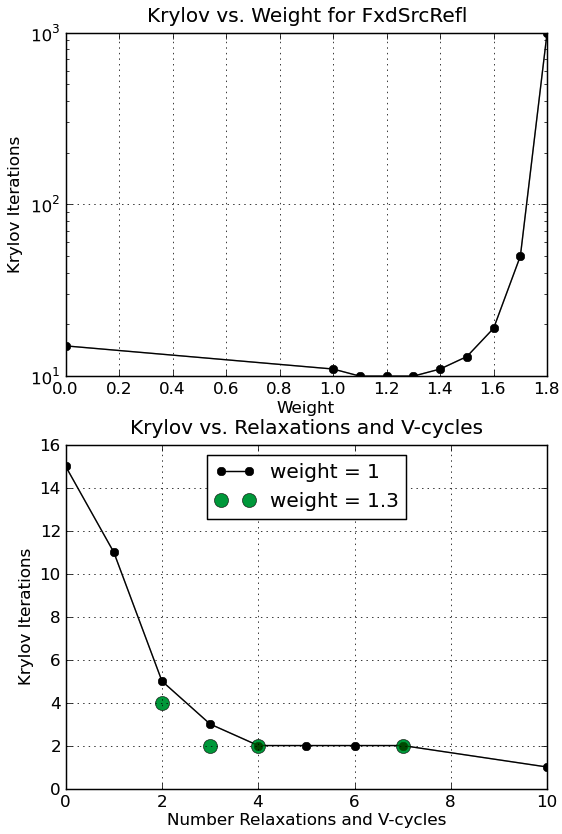
\includegraphics [width=0.7\textwidth, height=0.8\textheight] {FxdSrcRefl}
   \end{center}
   \caption{Small Fixed Source Problem with Reflecting Boundaries, Preconditioning Parameter Studies}
   \label{fig:FxdSrcRefl}
\end{figure}

The behavior of this problem is similar to but slightly different from the vacuum case. The weight variation again decreases the number of iterations initially and then increases dramatically. There is no ``sweet spot'' in this case, and 1,000 iterations is reached at $w1.8$ rather than $w2.1$. The $r$ and $v$ study showed two things. One is that early on a higher weight of 1.3 was better than a weight of 1. The other was that eventually the number of iterations can be decreased to 1. 

These results confirm that increasing $r$ and/or $v$ decrease Krylov iteration count. They also indicate that using a small amount of weight is beneficial, but a large amount is not. Neither of these problems exhibited the problems with a weight over 1 at low $r$ and $v$. All of these test problems were very small and simple. Testing with larger and more complex problems is needed as well. 

%-------------------------------------------------------------------------------------------------------
%-------------------------------------------------------------------------------------------------------
\subsubsection{Fixed Source Solver and Angle Comparisons} 
Another fixed source problem was the half iron, half graphite, toy problem from Chapter~\ref{sec:Chp2}. For this calculation a grid of 10 $\times$ 10 $\times$ 10 was used with $S_{8}$ and $P_{0}$. The tolerance and upscatter tolerance were 1 $\times$ 10$^{-6}$. This problem had vacuum boundaries and 27 energy groups, 13 of which have upscattering. A few calculations were done with this setup to investigate the number of iterations with different solvers rather than the effect of preconditioning parameters. The results comparing solvers can be seen in Table~\ref{table:FeC solvers}. 
%
\begin{table}[!h]
\caption{Iron Graphite Fixed Source Cube, Solver and Preconditioning Comparison}
\begin{center}
\begin{tabular}{l c l c}
\hline
Solver & GS iters & Krylov & time (s)\\[0.5ex]
\hline
GS &  12 & 1,727 & 1.12 $\times 10^{2}$ \\
GS TTG & 11 & 1,687 & 1.99 $\times 10^{2}$  \\
MG Krylov & n/a & 30 & 8.78 $\times 10^{1}$ \\
w1 r2 v2 & n/a & 10 & 7.07 $\times 10^{2}$ \\
w1.3 r4 v4 & n/a & 4 & 1.29 $\times 10^{3}$ \\
\hline
\end{tabular}
\end{center}
\label{table:FeC solvers}
\end{table}

Preconditioning reduced the number of Krylov iterations dramatically for this problem, which contains highly scattering material. While the Krylov subspace sizes are made from smaller vectors when GS is used, all the problems using MG Krylov took many fewer iterations. The highly preconditioned problem needed 4 Krylov iterations while unaccelerated Gauss Seidel needed 1,727.  

The timing comparison is not so favorable. With the unoptimized state of the preconditioner, using it for fixed source problems increases rather than decreases run time. Even though many fewer Krylov iterations are taken, the overall preconditioned run times are longer than all other calculations. This may not be the best problem for examining timing, however. Accelerated GS was slower than unaccelerated GS, which is not typical.

The option of using a different angle set within the preconditioner was investigated very briefly. The overall problem was solved with $S_{8}$, but the preconditioner used $S_{2}$. For the $w1r2v2$ case the time was reduced from 7.07 $\times 10^{2}$ seconds to 1.57 $\times 10^{2}$ seconds, a factor of 4.5. With the smaller angle set in the multigrid method the solve time was less than accelerated GS. 

%-------------------------------------------------------------------------------------------------------
%-------------------------------------------------------------------------------------------------------
\subsubsection{RQI Intermediate Problem}
The intermediately-sized infinite medium problem from Chapter~\ref{sec:Chp3} that has 27 groups and a very small dominance ratio was solved with preconditioned RQI. This is the first test to see if the preconditioner can converge the Krylov iterations when they did not converge with it. Recall that RQI was originally unable to converge the eigenvector for this problem, but got an eigenvalue close to the correct answer. The results with the preconditioner are shown in Table~\ref{table:impi RQI}. Like all the problems discussed so far, this was solved without any parallelization using the debug version of Denovo and GMRES. 
%
\begin{table}[!h]
\caption{Intermediate Problem With Rayleigh Quotient Iteration, Preconditioning Results}
\begin{center}
\begin{tabular}{c c c l l c c}
\hline
Weight & Relaxations & V-cycles & $k$ & Krylov & RQI & Time (s) \\[0.5ex]
\hline
0    & 0 & 0 & 0.397 & 39,025                  & 40$^{*}$  & 5.43 $\times 10^{4}$ \\
1    & 1 & 1 & 0.398 & 3,014$^{\dagger}$  & 4 & 2.66 $\times 10^{4}$ \\
1    & 3 & 1 & 0.398 & 50                        & 3 & 1.03 $\times 10^{4}$ \\
1    & 4 & 1 & 0.398 & 44$^{\dagger}$      & 3 & 1.16 $\times 10^{3}$ \\
1    & 2 & 2 & 0.398 & 44$^{\dagger}$      & 3 & 2.86 $\times 10^{2}$ \\
1    & 4 & 4 & 0.4     & 16                       & 3 & 1.99 $\times 10^{3}$ \\
1    & 5 & 4 & 0.4     & 14$^{\dagger}$     & 3 & 2.27 $\times 10^{2}$ \\
1.4 & 5 & 4 & -0.461 & 12$^{\dagger}$     & 2 & 1.74 $\times 10^{3}$ \\
1    & 5 & 5 & 0.4     & 7$^{\dagger}$      & 2 & 1.58 $\times 10^{3}$ \\
\hline
1.1 & 4 & 1 & 0.398 & 43$^{\dagger}$      & 3 & 1.16 $\times 10^{3}$ \\
1.1 & 1 & 4 & 0.398 & 43$^{\dagger}$      & 3 & 1.35 $\times 10^{3}$ \\
1.1 & 2 & 2 & 0.398 & 43$^{\dagger}$      & 3 & 1.18 $\times 10^{3}$ \\
\hline
0.7 & 1 & 1 & 0.399 & 3,001$^{\dagger}$ & 4 & 2.25 $\times 10^{4}$ \\
0.7 & 3 & 1 & 0.4    & 87$^{\dagger}$      & 5 & 1.95 $\times 10^{3}$ \\
0.7 & 3 & 3 & 0.4    & 47$^{\dagger}$      & 5 & 2.92 $\times 10^{3}$ \\
0.4 & 3 & 1 & \# & \#$^{\dagger}$      & \# & \# $\times 10^{3}$ \\
\hline 
\end{tabular}\\
$^{*}$terminated manually\\
$^{\dagger}$negative flux with correct magnitude
\end{center}
\label{table:impi RQI}
\end{table}

This calculation had a lot of issues. Most of the time the flux was correct in magnitude, but negative. It may be that for this problem the shift became negative and created a negative eigenvector that was the right magnitude. Another concern is that when the problem was heavily preconditioned, the eigenvector converged but gave a negative and incorrect eigenvalue. 

In addition, the correct eigenvalue was almost never calculated. The reported eigenvalues are always within at least 2.03 $\times 10^{-3}$ of the reference, but the $k$ tolerance was supposed to be $1 \times 10^{-5}$. T

here was only one test where the correct eigenvalue and positive correct eigenvector were found. A serious concern about these behaviors is that the method gives no warning or indication that something has gone awry until the negative eigenvector/value is reported at the end of the calculation. 

At this time it is unknown why preconditioned RQI had such a hard time with this calculation. Preconditioned RQI did have more trouble with the small reflecting problem than the vacuum problem. Perhaps the characteristics of $\ve{A}$ for this problem are just quite difficult. Whatever the reason, RQI did not perform well on this problem regardless of whether it was preconditioned.  

Some parameter information can still be gleaned from this study. The eigenvector did not converge after the first iteration when $w1r1v1$ was used. With more preconditioning the problem converged and the number of iterations was reduced. This is similar to what has been seen before. However, when a lot of preconditioning was used, the problem did not get the right eigenvalue. This is a behavior that was not observed in the simpler problems. 

These numbers further confirm that it is the total number of relaxations done, not the specific combination of $r$ and $v$, that determine the reduction in iteration count. That is, $r1v4$ = $r4v1$ = $r2v2$; though there is a difference in timing. Using a larger $v$ and a smaller $r$ may be more time consuming than a smaller $v$ and a larger $r$. Doing more V-cycles requires more prolongation and restriction operations to transfer between grids whereas doing more relaxations per level does not. 

To investigate whether some of the strange behavior was coming from GMRES, this problem was also attempted with BiCGSTAB. The preconditioning was set to $r2v2$, and the weight was increased in 0.1 increments from 1.0 to 1.5. In the cases where the calculation terminated itself, it was because a negative eigenvalue was found (which automatically ends the calculation) and the answers were incorrect. In the three cases where it didn't; $w1.1$, $w1.2$, $w1.3$; the problems were terminated manually. The eigenvalue was oscillating between a value close to the correct answer and a large number like 11. When a problem is terminated manually there is no way to obtain the flux, so it is unknown whether the flux was correct or not in those cases. Not only did BiCGSTAB not make the calculations better, it performed worse than GMRES.

The infinite medium problem was also solved with power iteration using no preconditioning and using a lot of preconditioning. Without preconditioning the problem took 180 Krylov iterations and $2.57 \times 10^{2}$ seconds. With $w1r5v5$ preconditioning it took 12 Krylov iterations and $2.19 \times 10^{3}$ seconds. Both calculations obtained an eigenvalue of 0.4 and a positive correct flux. Preconditioning substantially reduced the number of Krylov iterations needed. Further, the amount of preconditioning that worked with power iteration did not work with RQI. 

%-------------------------------------------------------------------------------------------------------
%-------------------------------------------------------------------------------------------------------
\subsubsection{2-D C5G7 Benchmark Study}
Next, the preconditioner was applied to the 2-D c5g7 benchmark using both PI and RQI with the goals of seeing if preconditioned RQI could converge the flux and $k$, to investigate the effect of preconditioning in both RQI and PI, and to see whether the lessons learned about preconditioning parameters still hold in a real problem. The problem used 16 cores on the small orthanc cluster at Oak Ridge: 4 x-blocks, 4 y-blocks, 1 z-block and 1 energy set. The total and upscattering tolerances were 1 $\times 10^{-3}$, with a $k$ tolerance of 1 $\times 10^{-5}$. An optimized version of Denovo was used.  

A weight variation study was done with power iteration first. The results using $r1v1$ are shown in Figure~\ref{fig:2-Dc5g7PI}. The data that is plotted can be found in Appendix~\ref{sec:AppendixD}, Table~\ref{table:2-D c5g7}. All $k$ values were within the uncertainty of the benchmark and so are not reported. All preconditioned cases needed 31 power iterations while the unpreconditioned case took 32.
%
\begin{figure}[!ht]
    \begin{center}
      \includegraphics [width=0.7\textwidth, height=0.7\textheight] {2dc5g7PI}
   \end{center}
   \caption{2-D C5G7 Benchmark, Preconditioner Weight Variation With Power Iteration}
   \label{fig:2-Dc5g7PI}
\end{figure}

This study shows the preconditioner is very effective at reducing the number of Krylov iterations used by power iteration. The unpreconditioned case took 3,129 MG Krylov iterations.. As the weight was increased from 1 to 1.4, the number of Krylov iterations and the time to solution both decreased. With $w1.4$, 1,458 MG Krylovs were taken. The time and iteration count both went back up with a weight of 1.5. When the weight was increased beyond 1.5 none of the multigroup iterations converged, and the problem was terminated manually after several power iterations. 

Two other calculations with a higher level of preconditioning were also done. When the parameters were $w1.4r2v2$ the number of Krylov iterations were reduced to 438 and the calculation took 1.77 $\times 10^{4}$ seconds, both lower than all the cases using $r1v1$. For $w1r3v3$, 253 Krylov iterations and 2.28 $\times 10^{4}$ seconds were required. This had the smallest number of Krylov iterations, but a slightly longer time than all the calculations except $w1.5r1v1$.	

The results from the RQI study are in Table~\ref{table:2-D c5g7 rqi}. ``Krylov'' is the total number of Krylov iterations and ``RQI'' is the total number of Eigenvalue iterations. In all cases, except the unpreconditioned one, $k$ was within the uncertainty of the benchmark value. The ``$<$ 1,000?'' column indicates whether or not the multigroup iterations converged during the RQI process. If the value is ``no'' that means the eigenvector only converged during the first iteration. A number indicates the last eigenvalue iteration for which the Krylov method took less than 1,000 iterations. A ``yes'' means all of the Krylov iterations converged.
%
\begin{table}[!h]
\caption{2-D C5G7 Benchmark, Convergence Study With Rayleigh Quotient Iteration}
\begin{center}
\begin{tabular}{c c c l c c c}
\hline
Weight & Relaxations & V-cycles & Krylov & RQI & $<$ 1,000? & Time (s) \\[0.5ex]
\hline
0    & 0 & 0 & 119,006 & 120$^{*}$ & no &9.38 $\times 10^{4}$ \\
1    & 1 & 1 & 16,007   & 17            & no & 2.02 $\times 10^{5}$ \\
1.2 & 1 & 1 & 40,008   & 41$^{*}$   & no & 2.06 $\times 10^{5}$ \\
1    & 3 & 1 & n/a         & n/a$^{*}$  & 7   & n/a \\
1    & 2 & 2 & 11,158   & 19            & alternated & 3.99 $\times 10^{5}$ \\
1    & 3 & 2 & 3,320     & 19            & 14 & 1.64 $\times 10^{5}$ \\
\hline
1    & 3 & 3 & 299        & 19            & yes & 2.57 $\times 10^{4}$ \\
1.1 & 3 & 3 & 281        & 19            & yes & 2.40 $\times 10^{4}$ \\
1.3 & 3 & 3 & 254        & 19            & yes & 2.19 $\times 10^{4}$ \\
1.5 & 3 & 3 & n/a         & n/a$^{*}$ & no & n/a \\
\hline 
\end{tabular} \\
$^{*}$terminated manually
\end{center}
\label{table:2-D c5g7 rqi}
\end{table}
%

These results show a few important things. It seems that preconditioning can hold RQI on track enough to get the right eigenvalue when the eigenvector is not quite converging, like what happened with the unpreconditioned infinite medium problem. For many of the calculations the eigenvector didn't converge, or didn't converge all the time, but the correct eigenvalue was still found (even in the $w1.2r1v1$ case that was terminated manually). As the preconditioning increased, the eigenvector came closer to converging for all iterations. 

Most importantly, with enough preconditioning the eigenvector within RQI can be converged and the right eigenpair can be found. For the first three $w\#r3v3$ cases all of the Krylov iterations converged. As a result, the calculation time decreased by an order of magnitude compared to the ones where they did not converge every time. If the Krylov iterations did converge, increasing the weight decreased iteration count and wall time for small weights. As in other problems, too much weight caused the calculation not to converge at all. This test case was the first to demonstrate that the preconditioner can get RQI to converge. 

Only the $w1r3v3$ calculation overlap between RQI and PI. PI took fewer Krylov iterations and less time, though RQI used fewer eigenvalue iterations. The RQI problem was also tried with BiCGSTAB as the Krylov solver for an unpreconditioned case and a $w1r3v3$ case. Every multigroup iteration went to the 1,000 iteration limit and the problem was terminated manually after several RQ iterations.

%-------------------------------------------------------------------------------------------------------
%-------------------------------------------------------------------------------------------------------
 \subsubsection{3-D C5G7 Benchmark Study}
The preconditioner using both PI and RQI was also applied to the 3-D c5g7 benchmark with an optimized version of Denovo. The goals of this study were essentially the same as the 2-D study, except that this problem is larger, and the first to approach a real ``grand challenge''-type of calculation. This time the medium-sized oic cluster at Oak Ridge was used and each problem was given 720 cores with 40 x-blocks, 18 y-blocks and 5 z-blocks. The total and upscattering tolerances were 1 $\times 10^{-4}$, with a $k$ tolerance of 1 $\times 10^{-5}$ unless otherwise indicated. 

The power iteration results are in Table~\ref{table:3-D c5g7}. None of the $k$s were within the uncertainty bounds of the reported benchmark; all results were low by about 0.011. The wall time limit was 12 hours. 
%
\begin{table}[!h]
\caption{3-D C5G7 Benchmark, Preconditioning Parameter Scoping With Power Iteration}
\begin{center}
\begin{tabular}{c c c c l l}
\hline
Weight & Relaxations & V-cycles & Krylov & PI & Time (s) \\[0.5ex]
\hline
0    & 0 & 0 & 1,224 & 32 & 4.46 $\times 10^{3}$ \\
1    & 1 & 1 & 708    & 32 & 2.12 $\times 10^{4}$ \\
1.2 & 1 & 2 & 448    & 32 & 2.38 $\times 10^{4}$ \\
1.2 & 2 & 1 & 448    & 32 & 2.39 $\times 10^{4}$ \\
1.3 & 2 & 2 & 288    & 32 & 2.84 $\times 10^{4}$ \\
1    & 3 & 3 & 126    & 14$^{*}$  & 4.04 $\times 10^{4}$ \\
1.5 & 3 & 3 & 192    & 32 & 3.73 $\times 10^{4}$ \\
1    & 4 & 4 & n/a     & n/a          & exceeded wall time \\
1    & 4 & 4 & n/a     & n/a$^{*}$ & exceeded wall time \\
1.5 & 5 & 5 & n/a     & n/a          & exceeded wall time \\
\hline 
\end{tabular}\\
$^{*}$tol and upscatter tol = 1 $\times 10^{-5}$, $k$ tol = 1 $\times 10^{-3}$
\end{center}
\label{table:3-D c5g7}
\end{table}

The 3-D benchmark study shows the preconditioner can reduce the number of required Krylov iterations substantially for challenging problems. There was no effect on the number of eigenvalue iterations for a given tolerance set. The effect of preconditioning parameters was consistent with what was observed in other calculations. However, using large values for $r$ and $v$ made the calculation take too long to get results. On the oic machine, if a calculation exceeds wall time there is no way to get any of the results from the scratch space. Therefore, no conclusions can be drawn from this problem about the effect of substantial preconditioning when using power iteration for a real, 3-D problem. 

The degree to which the RQI-computed $k$ matched the benchmark was the same as PI: within 0.011 when the tighter calculation tolerance was used, but not within the reported uncertainty. The results are in Table~\ref{table:3-D c5g7 rqi}. The maximum wall time was 12 hours here as well. 
%
\begin{table}[!h]
\caption{3-D C5G7 Benchmark, Preconditioning Parameter Scoping With Rayleigh Quotient Iteration}
\begin{center}
\begin{tabular}{c c c c l l}
\hline
Weight & Relaxations & V-cycles & Krylov & RQI & Time (s) \\[0.5ex]
\hline
0    & 0 & 0 & n/a     & n/a          & exceeded wall time \\
1    & 1 & 1 & n/a     & n/a          & exceeded wall time \\
1.5 & 1 & 1 & n/a     & n/a          & exceeded wall time \\
1.2 & 2 & 1 & n/a     & n/a          & exceeded wall time \\
1.3 & 2 & 2 & 302    & 19           & 2.32 $\times 10^{4}$ \\
1    & 3 & 3 & 103    & 9$^{*}$    & 3.02 $\times 10^{4}$ \\
1    & 3 & 3 & 164    & 15$^{\dagger}$ & 3.38 $\times 10^{4}$ \\
1.5 & 3 & 3 & 187    & 19           & 3.24 $\times 10^{4}$ \\
1    & 4 & 4 & n/a     & n/a          & exceeded wall time \\
1    & 4 & 4 & 74     & 9$^{*}$    & 2.29 $\times 10^{4}$ \\
1.5 & 5 & 5 & n/a     & n/a          & exceeded wall time \\
\hline 
\end{tabular}\\
$^{*}$tol and upscatter tol = 1 $\times 10^{-5}$, $k$ tol = 1 $\times 10^{-3}$\\
$^{\dagger}$tol and upscatter tol = 1 $\times 10^{-4}$, $k$ tol = 5 $\times 10^{-5}$
\end{center}
\label{table:3-D c5g7 rqi}
\end{table}  

A few things are going on here. What is likely happening when the problems with lower parameter values run out of time is that the eigenvector is not converging. As was seen before, the calculations take a long time when every eigenvalue iteration uses 1,000 Krylov iterations. Unfortunately, there is no way to confirm this theory or find out if the eigenvalue is close to correct since the output cannot be obtained. 

With an intermediate amount of preconditioning, RQI converged and performed better than the analogous PI cases. There are three cases where both problems finish and the same tolerances were used: $w1.3r2v2$, $w1r3v3$, $w1.5r3v3$. In all three RQI takes less time and fewer eigenvalue iterations. In the second two it also takes fewer Krylov iterations. RQI even finishes in time for the $w1r4v4$ calculation when PI did not. 

The 3-D benchmark problem shows that for at least some problems, preconditioned RQI converges more quickly in all senses than PI. It is pertinent that the case for which this is true is the most interesting problem shown. It seems that RQI can only be successful if it is preconditioned enough to get the eigenvector to converge. Finally, these results continue to confirm that a small amount of weight works well. Increasing $r$ and $v$ decrease iteration count, but at what can be a high time cost. An intermediate amount of preconditioning will likely provide the best balance of reduced iteration count for the time invested once the preconditioner is optimized. 

%-------------------------------------------------------------------------------------------------------
%-------------------------------------------------------------------------------------------------------
\subsubsection{Multisets}
The last, but certainly not least, area of investigation was how the preconditioner faired when using multisets. To investigate the effect of multigrid in energy with multisets on the Krylov iterations without worrying about impacts of an eigenvalue calculation, the iron graphite fixed source problem was considereded first. This was run on orhtanc using an optimized version of the code. All previous parameter studies were used to pick preconditioning values that were likely to work well. 

To make the problem large enough to be able to use energy sets, the grid was increased to $50 \times 50 \times 50$, though $S_{4}$ was used instead of $S_{8}$. The unpreconditioned version was compared to one with $w1r2v2$ on 1 to 10 sets. Note that with 27 groups, 10 sets is the maximum possible to still be able to use the preconditioner. In addition, 2 x-blocks, 2 y-blocks, and 1 z-block were used. The calculations therefore used between 4 and 40 cores. With all set combinations the preconditioned calculation took 27 GMRES iterations while the unpreconditioned took 123.

Because the number of iterations did not change with sets, the only thing to compare was time. The focus is on relative change in time rather than absolute time since there is still room for the preconditioner to be optimized. Three plots are shown in Figure~\ref{fig:FeC multisets}. From the top, the first shows the wall time for the preconditioned and unpreconditioned (``regular'') calculations as a function of time. The second plots the ratio of the calculation time with N sets to the time with 1 set. The last plot is of the relative difference between the two times. The data that is plotted can be found in Appendix~\ref{sec:AppendixD}, Table~\ref{table:FeC multisets}.
%
\begin{figure}[!ht]
    \begin{center}
      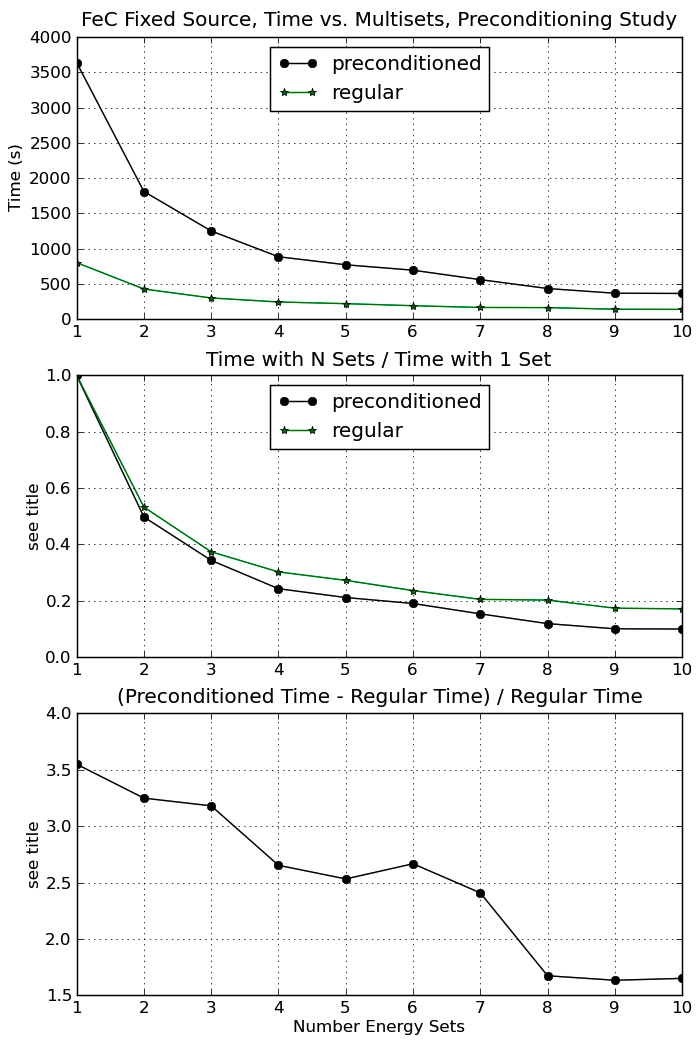
\includegraphics [width=0.7\textwidth, height=0.8\textheight] {FeCmultisets}
   \end{center}
   \caption{Iron Graphite Fixed Source Problem, Preconditioner Multiset Study}
   \label{fig:FeC multisets}
\end{figure}

The 1 set wall time without preconditioning was 8.00 $\times 10^{3}$ seconds and the 10 set time was 1.34 $\times 10^{3}$ seconds. Without preconditioning a 10 fold increase in computing power gave about a 6 fold decrease in run time. With preconditioning the 1 set time was 3.64 $\times 10^{3}$ and the 10 set time was 3.63 $\times 10^{2}$. The scaling in this case was nearly one to one.

This test was also run with increased preconditioning parameters for 1 set and 10 sets to see if that made a difference. The angle set was changed back to $S_{8}$ and there was no decomposition in space. With $w1.3r4v4$ the number of Krylov iterations decreased to 11. With 1 set this took 6.49 $\times 10^{4}$ sec to complete. With 10 sets this was reduced to 5.02 $\times 10^{3}$ sec. A 10 fold increase in computing power gave more than a 10 fold decrease in run time. Without preconditioning the 1 set wall time was 8.81 $\times 10^{3}$ seconds and the 10 set time was 1.04 $\times 10^{3}$ seconds, again less than one-to-one scaling.

The infinite medium, 27 group problem was also used to study how the preconditioner faired with energy set decomposition. Because this problem has reflecting boundary conditions it could only be used with power iteration (recall, RQI cannot do multisets with reflecting boundaries at this time). These calculations were also done on orthanc, using between 1 and 10 sets and an optimized version of the code. No other problem settings were changed from what was presented above. 

When the preconditioning parameters were $w1r2v2$, the Krylov iterations were reduced from 180 (90 Krylov per PI with 2 PI) to 46 (23 Krylov per PI with 2 PI). Three plots are shown in Figure~\ref{fig:impi multisets}, they are of the same trends as the iron graphite cube plot. A table of the data can be found in Appendix~\ref{sec:AppendixD}, Table~\ref{table:impi multisets}.
%
\begin{figure}[!ht]
    \begin{center}
      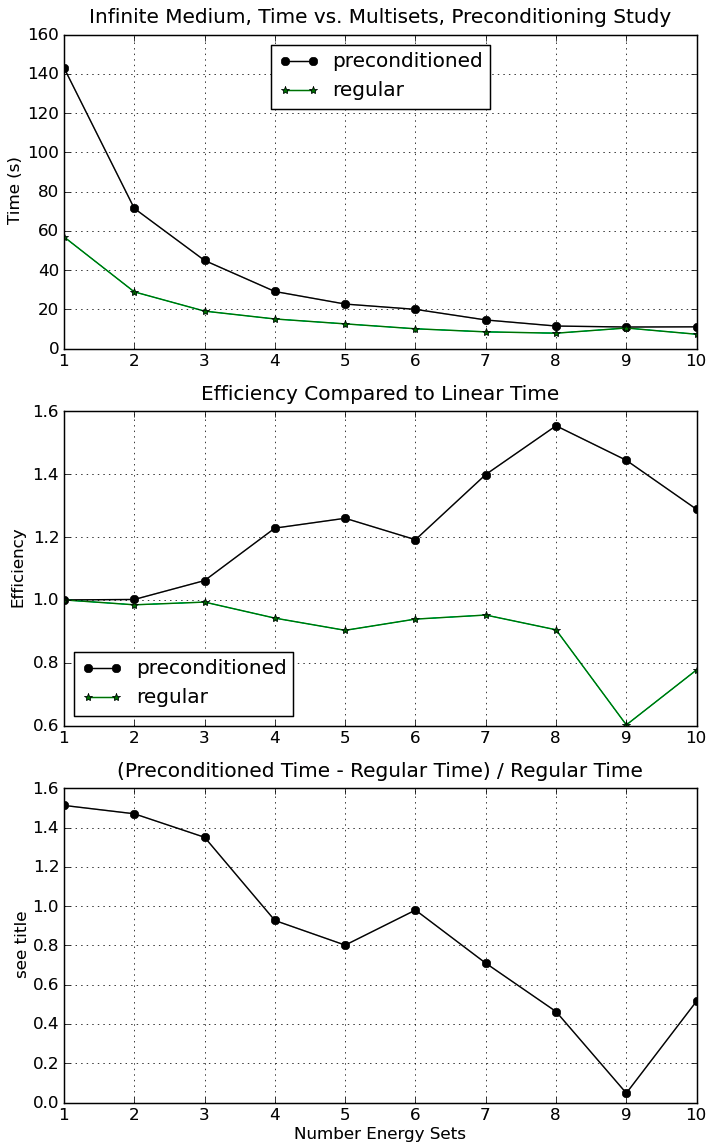
\includegraphics [width=0.7\textwidth, height=0.8\textheight] {impimultisets}
   \end{center}
   \caption{Infinite Medium Eigenvalue Problem, Preconditioned Multiset Study with Power Iteration}
   \label{fig:impi multisets}
\end{figure}

This test was run with increased preconditioning parameters for 1 set and 10 sets as well. The number of Krylov iterations decreased to 8 per eigenvalue iteration, with 2 eigenvalue iterations when $w1r4v4$ was used. With 1 set this took 4.02 $\times 10^{2}$ seconds to complete. With 10 sets this was reduced to 2.94 $\times 10^{1}$ seconds. For this preconditioning set, too, a 10 fold increase in computing power gave more than a 10 fold decrease in run time. When the problem was not preconditioned and used 1 set, the wall time was 56.9 seconds; with 10 sets it was 7.32 seconds. Once again, without preconditioning a 10 fold increase in computing power gave less than a 10 fold decrease in run time. 
 
Finally, the Full PWR900 problem was calculated using both power iteration and Rayleigh quotient iteration on the Jaguar machine with multisets and preconditioning. The large PWR problem is the illustrative example of using all the new methods in combination. This test uses the multigroup Krylov solver to decompose the calculation in energy, the eigenvalue problem is solved with Rayleigh quotient iteration, and the whole thing is preconditioned with the parallelized multigrid in energy. It is also exactly the kind of large and challenging problem this work is designed to solve. %This is the only large scale eigenvalue test with all vacuum boundary conditions, and therefore the only one that could use multisets with RQI. 

The 44-group, 1.7 trillion unknown version of the problem was used for this scaling study. The tolerance and $k$ tolerance were 1 $\times 10^{-3}$, and the upscattering tolerance was 1 $\times 10^{-4}$. The preconditioner settings were $w1r3v3$, and 1, 4, 11, and 22 sets were used. There were 578 $\times$ 578 $\times$ 700 mesh elements. With 22 sets, 96 x-blocks, 94 y-blocks, and 10 z-blocks were used. All other cases had 102 x-blocks, 100 y-blocks, and 10 z-blocks. All of the results are in Table~\ref{table:full PWR}. 
%
\begin{table}[!h]
\caption{Full PWR, Preconditioned Strong Scaling Study}
\begin{center}
\begin{tabular}{l c c c l c c l}
\hline
Solver & Sets & Cores & $k$ & Krylov & Eigenvalue & Total (min) & Solver (min)\\[0.5ex]
\hline
RQI & 1   & 10,200   &  &   &                   &  &  \\
PI    & 1   & 10,200   &  &  &       &  &  \\
RQI & 4   & 40,800   & 1.269 & 76   &  6               & 802.60 & 801.32 \\
PI    & 4   & 40,800  &  &  &  &  &  \\
RQI & 11 & 112,200 & 1.269 & 76   & 6                & 331.43 & 330.38 \\
PI    & 11 & 112,200 & 1.270 & 111 & 11$^{\dag}$ & 480.63 & n/a \\
RQI & 22 & 198,528 & 1.269 & 76   & 6                & 143.62 & 142.56 \\
PI    & 22 & 198,528 & 1.271 & 161 & 16$^{*}$      & 285.92 & n/a \\
\hline 
\end{tabular}\\
$^{*}$machine taken down for maintenance during calculation \\
$^{\dag}$exceeded wall time limit of 480 minutes
\end{center}
\label{table:full PWR}
\end{table}  

Comparison between PI and RQI with 11 and 22 sets is difficult because PI did not finish in either case. However, both clearly show that RQI is much faster and requires far fewer iterations than PI for this problem. In the 11 set case the author failed to choose a large enough wall time limit. Because RQI, which was run first, finished in about 5.5 hours, a wall time for PI of 8 hours was selected. In previous problems the solve time for PI was close to or faster than RQI, so 8 hours seemed reasonable. Partway through the 22 set calculation a portion of the jaguar machine was taken offline leaving only 162,240 cores, so the calculation was terminated. Nevertheless, the partial results are still informative. 

A few key conclusions can be drawn from the multiset studies about the tradeoff between the number of groups per set and about the overall usefulness of the multigrid in energy method with multisets. An important observation is that the number of GMRES iterations did not change with the number of sets. This means convergence improvement from the preconditioner does not come from the depth of V-cycle. Only going down 1 or 2 grids had as much of an impact as going down something like 6. This indicates it is not necessary to coarsen down to one group. 

Preconditioning gives better than one-to-one scaling in energy. This is because as the number of sets increases the total number of Krylov iterations remains constant while each application of the preconditioner becomes less costly. The preconditioning cost goes down because the V-cycle becomes shallower. That is, each application of the preconditioner is doing fewer total relaxations and is therefore less expensive. Once the preconditioner is optimized this may become less super-linear since it will take a smaller total fraction of the runtime. The scaling will also be less impressive if the preconditioner is modified to always use two grids instead of going down to one energy group. 

\subsubsection{Summary of Findings}
All of the test results lead to some useful conclusions. In terms of preconditioning parameters, increasing $r$ and/or $v$ almost always decreases Krylov iteration count and sometimes decreased eigenvalue iteration count. $r$ and $v$ have equal effect in the preconditioner because they determine the total number of relaxations. All of the relaxations can be executed via $r$ or $v$ or some combination. The way the relaxations are distributed between $r$ and $v$ may influence the calculation time. It seems that using a larger $r$ than $v$ is the best choice as it minimizes prolongation and restriction operations. 
 
Increasing the weight a small amount, up to about 1.3 or 1.4, is generally beneficial. However, using a large weight can be detrimental. Weight is the least consistent parameter, behaving differently in different problems with different degrees of preconditioning. Using a weight of 1 with small $r$ and $v$ and a weight of between 1 and 1.3 for an intermediate $r$ and$v$ is probably the safest approach. 

Overall, a moderate amount of preconditioning seems to give the best payoff. A little bit of preconditioning does not do enough, and a lot is not worth the extra run time. This is related to the fact that the improvement gained from preconditioning is non-linear; doubling the preconditioning parameters does not necessarily halve the iteration count. This means the impact of preconditioning parameters can not be accurately predicted ahead of time. 

Some lessons were also learned about preconditioner choices besides $w$, $r$, and $v$. Using the reduced angular expansion option within the preconditioner may have a lot of pay off. This option must be turned on by the user, and should be exploited when possible. The shifted operator is definitely a bad idea with reflecting boundaries and is probably a bad idea in general. The default behavior is to use the unshifted operator. GMRES, which is the default Krylov method, should always be selected over BiCGSTAB. Based on the multiset results, the depth of the V-cycles should probably be set to only one or two levels. Implementing this choice requires changing the code itself. An option could be added to give the user more control over this setting.

%-------------------------------------------------------------------------------------------------------
\subsection{Implications}
There were two primary motivations for the multigrid in energy preconditioner. The traditional eigenvalue solver power iteration can be slow for systems with high dominance ratios, which motivated the use of RQI. As was found in Chapter~\ref{sec:Chp3}, Krylov methods stagnate for poorly conditioned systems such as those created by RQI. Preconditioning is therefore required to be able to use RQI for real problems. 

In addition, ever-expanding computers allow codes to use hundreds of thousands or cores for large computations. Any new preconditioner in Denovo must be able to use these machines efficiently. At its core, the multigroup in energy preconditioner is designed to take advantage of energy parallelization. The way it has been implemented, the multigrid in energy method does not require any inter-set communication so it should scale extremely well. The new energy decoupling provided by the MG Krylov solver is what allows this preconditioner to be parallelized in energy. Without that, the preconditioner would not be as attractive. 

Using a multigrid method in the energy domain is new for the neutron transport equation. The author was unable to find a similar idea in the literature. This is not surprising because the motivation for the preconditioner is relatively new as well. Only in the last few years have energy parallelization and Rayleigh quotient iteration become feasible. Without those drivers there was no reason to do multigrid in energy. 

The goals for the new preconditioner were to decrease iteration count for at least some problems, to enable RQI, and be decomposable in energy. All goals were achieved. The multigrid in energy preconditioner reduced the number of Krylov iterations for all problem types as long as the eigenvector converged. In a few cases it reduced the number of eigenvalue iterations. The preconditioner also makes RQI possible and scales to hundreds of thousands of cores without trouble. 











